% **************************************************************************************************************
% A Classic Thesis Style
% An Homage to The Elements of Typographic Style
%
% Copyright (C) 2017 André Miede and Ivo Pletikosić
%
% If you like the style then I would appreciate a postcard. My address
% can be found in the file ClassicThesis.pdf. A collection of the
% postcards I received so far is available online at
% http://postcards.miede.de
%
% License:
% This program is free software; you can redistribute it and/or modify
% it under the terms of the GNU General Public License as published by
% the Free Software Foundation; either version 2 of the License, or
% (at your option) any later version.
%
% This program is distributed in the hope that it will be useful,
% but WITHOUT ANY WARRANTY; without even the implied warranty of
% MERCHANTABILITY or FITNESS FOR A PARTICULAR PURPOSE.  See the
% GNU General Public License for more details.
%
% You should have received a copy of the GNU General Public License
% along with this program; see the file COPYING.  If not, write to
% the Free Software Foundation, Inc., 59 Temple Place - Suite 330,
% Boston, MA 02111-1307, USA.
%
% PLEASE SEE ALSO THE AUTHORS' NOTE REGARDING THIS LICENSE
% IN THE DOCUMENTATION (ClassicThesis.pdf --> Chapter 1 / Chapter01.tex)
% **************************************************************************************************************
\RequirePackage{silence} % :-\
    \WarningFilter{scrreprt}{Usage of package `titlesec'}
    %\WarningFilter{scrreprt}{Activating an ugly workaround}
    \WarningFilter{titlesec}{Non standard sectioning command detected}
\documentclass[ twoside,openright,titlepage,numbers=noenddot,headinclude,%1headlines,% letterpaper a4paper
                footinclude=true,cleardoublepage=empty,abstractoff, % <--- obsolete, remove (todo)
                BCOR=5mm,paper=a4,fontsize=11pt,%11pt,a4paper,%
                ngerman,american,%
                ]{scrreprt}

%********************************************************************
% Note: Make all your adjustments in here
%*******************************************************
% ****************************************************************************************************
% classicthesis-config.tex
% formerly known as loadpackages.sty, classicthesis-ldpkg.sty, and classicthesis-preamble.sty
% Use it at the beginning of your ClassicThesis.tex, or as a LaTeX Preamble
% in your ClassicThesis.{tex,lyx} with % ****************************************************************************************************
% classicthesis-config.tex
% formerly known as loadpackages.sty, classicthesis-ldpkg.sty, and classicthesis-preamble.sty
% Use it at the beginning of your ClassicThesis.tex, or as a LaTeX Preamble
% in your ClassicThesis.{tex,lyx} with % ****************************************************************************************************
% classicthesis-config.tex
% formerly known as loadpackages.sty, classicthesis-ldpkg.sty, and classicthesis-preamble.sty
% Use it at the beginning of your ClassicThesis.tex, or as a LaTeX Preamble
% in your ClassicThesis.{tex,lyx} with \input{classicthesis-config}
% ****************************************************************************************************
% If you like the classicthesis, then I would appreciate a postcard.
% My address can be found in the file ClassicThesis.pdf. A collection
% of the postcards I received so far is available online at
% http://postcards.miede.de
% ****************************************************************************************************


% ****************************************************************************************************
% 0. Set the encoding of your files. UTF-8 is the only sensible encoding nowadays. If you can't read
% äöüßáéçèê∂åëæƒÏ€ then change the encoding setting in your editor, not the line below. If your editor
% does not support utf8 use another editor!
% ****************************************************************************************************
\PassOptionsToPackage{utf8}{inputenc}
  \usepackage{inputenc}

% ****************************************************************************************************
% 1. Configure classicthesis for your needs here, e.g., remove "drafting" below
% in order to deactivate the time-stamp on the pages
% (see ClassicThesis.pdf for more information):
% ****************************************************************************************************
\PassOptionsToPackage{
  drafting=false,    % print version information on the bottom of the pages
  tocaligned=false, % the left column of the toc will be aligned (no indentation)
  dottedtoc=false,  % page numbers in ToC flushed right
  parts=true,       % use part division
  eulerchapternumbers=true, % use AMS Euler for chapter font (otherwise Palatino)
  linedheaders=false,       % chaper headers will have line above and beneath
  floatperchapter=true,     % numbering per chapter for all floats (i.e., Figure 1.1)
  listings=true,    % load listings package and setup LoL
  subfig=true,      % setup for preloaded subfig package
  eulermath=false,  % use awesome Euler fonts for mathematical formulae (only with pdfLaTeX)
  beramono=true,    % toggle a nice monospaced font (w/ bold)
  minionpro=false   % setup for minion pro font; use minion pro small caps as well (only with pdfLaTeX)
}{classicthesis}


% ****************************************************************************************************
% 2. Personal data and user ad-hoc commands
% ****************************************************************************************************
\newcommand{\myTitle}{A Classic Thesis Style\xspace}
\newcommand{\mySubtitle}{An Homage to The Elements of Typographic Style\xspace}
\newcommand{\myDegree}{Doktor-Ingenieur (Dr.-Ing.)\xspace}
\newcommand{\myName}{André Miede\xspace}
\newcommand{\myProf}{Put name here\xspace}
\newcommand{\myOtherProf}{Put name here\xspace}
\newcommand{\mySupervisor}{Put name here\xspace}
\newcommand{\myFaculty}{Put data here\xspace}
\newcommand{\myDepartment}{Put data here\xspace}
\newcommand{\myUni}{Put data here\xspace}
\newcommand{\myLocation}{Saarbrücken\xspace}
\newcommand{\myTime}{October 2017\xspace}
\newcommand{\myVersion}{version 4.4}

% ********************************************************************
% Setup, finetuning, and useful commands
% ********************************************************************
\newcounter{dummy} % necessary for correct hyperlinks (to index, bib, etc.)
\newlength{\abcd} % for ab..z string length calculation
\providecommand{\mLyX}{L\kern-.1667em\lower.25em\hbox{Y}\kern-.125emX\@}
\newcommand{\ie}{i.\,e.}
\newcommand{\Ie}{I.\,e.}
\newcommand{\eg}{e.\,g.}
\newcommand{\Eg}{E.\,g.}
% ****************************************************************************************************


% ****************************************************************************************************
% 3. Loading some handy packages
% ****************************************************************************************************
% ********************************************************************
% Packages with options that might require adjustments
% ********************************************************************
%\PassOptionsToPackage{ngerman,american}{babel}   % change this to your language(s), main language last
% Spanish languages need extra options in order to work with this template
\PassOptionsToPackage{spanish,es-lcroman, es-tabla}{babel}
    \usepackage{babel}

\usepackage{csquotes}
\PassOptionsToPackage{%
  %backend=biber,bibencoding=utf8, %instead of bibtex
  backend=bibtex8,bibencoding=ascii,%
  language=auto,%
  style=numeric-comp,%
  %style=authoryear-comp, % Author 1999, 2010
  %bibstyle=authoryear,dashed=false, % dashed: substitute rep. author with ---
  sorting=none, % name, year, title
  maxbibnames=10, % default: 3, et al.
  %backref=true,%
  natbib=true % natbib compatibility mode (\citep and \citet still work)
}{biblatex}
    \usepackage{biblatex}
    
\PassOptionsToPackage{fleqn}{amsmath}       % math environments and more by the AMS
  \usepackage{amsmath}

% ********************************************************************
% General useful packages
% ********************************************************************
\PassOptionsToPackage{T1}{fontenc} % T2A for cyrillics
  \usepackage{fontenc}
\usepackage{textcomp} % fix warning with missing font shapes
\usepackage{scrhack} % fix warnings when using KOMA with listings package
\usepackage{xspace} % to get the spacing after macros right
\usepackage{mparhack} % get marginpar right
%\usepackage{fixltx2e} % fixes some LaTeX stuff --> since 2015 in the LaTeX kernel (see below)
% \usepackage[latest]{latexrelease} % emulate newer kernel version if older is detected
\PassOptionsToPackage{printonlyused,smaller}{acronym}
  \usepackage{acronym} % nice macros for handling all acronyms in the thesis
  %\renewcommand{\bflabel}[1]{{#1}\hfill} % fix the list of acronyms --> no longer working
  %\renewcommand*{\acsfont}[1]{\textsc{#1}}
  %\renewcommand*{\aclabelfont}[1]{\acsfont{#1}}
  %\def\bflabel#1{{#1\hfill}}
  \def\bflabel#1{{\acsfont{#1}\hfill}}
  \def\aclabelfont#1{\acsfont{#1}}
% ****************************************************************************************************
%\usepackage{pgfplots} % External TikZ/PGF support (thanks to Andreas Nautsch)
%\usetikzlibrary{external}
%\tikzexternalize[mode=list and make, prefix=ext-tikz/]
% ****************************************************************************************************


% ****************************************************************************************************
% 4. Setup floats: tables, (sub)figures, and captions
% ****************************************************************************************************
\usepackage{tabularx} % better tables
  \setlength{\extrarowheight}{3pt} % increase table row height
\newcommand{\tableheadline}[1]{\multicolumn{1}{c}{\spacedlowsmallcaps{#1}}}
\newcommand{\myfloatalign}{\centering} % to be used with each float for alignment
\usepackage{caption}
% Thanks to cgnieder and Claus Lahiri
% http://tex.stackexchange.com/questions/69349/spacedlowsmallcaps-in-caption-label
% [REMOVED DUE TO OTHER PROBLEMS, SEE ISSUE #82]
%\DeclareCaptionLabelFormat{smallcaps}{\bothIfFirst{#1}{~}\MakeTextLowercase{\textsc{#2}}}
%\captionsetup{font=small,labelformat=smallcaps} % format=hang,
\captionsetup{font=small} % format=hang,
\usepackage{subfig}
% ****************************************************************************************************


% ****************************************************************************************************
% 5. Setup code listings
% ****************************************************************************************************
\usepackage{listings}
%\lstset{emph={trueIndex,root},emphstyle=\color{BlueViolet}}%\underbar} % for special keywords
\lstset{language=[LaTeX]Tex,%C++,
  morekeywords={PassOptionsToPackage,selectlanguage},
  keywordstyle=\color{RoyalBlue},%\bfseries,
  basicstyle=\small\ttfamily,
  %identifierstyle=\color{NavyBlue},
  commentstyle=\color{Green}\ttfamily,
  stringstyle=\rmfamily,
  numbers=none,%left,%
  numberstyle=\scriptsize,%\tiny
  stepnumber=5,
  numbersep=8pt,
  showstringspaces=false,
  breaklines=true,
  %frameround=ftff,
  %frame=single,
  belowcaptionskip=.75\baselineskip
  %frame=L
}
% ****************************************************************************************************


% ****************************************************************************************************
% 6. PDFLaTeX, hyperreferences, and citation backreferences
% ****************************************************************************************************
% ********************************************************************
% Using PDFLaTeX
% ********************************************************************
\PassOptionsToPackage{hyperfootnotes=false,pdfpagelabels}{hyperref}
  \usepackage{hyperref}  % backref linktocpage pagebackref
%\ifpdf
%\pdfcompresslevel=9
%\pdfadjustspacing=1
%\fi
%\PassOptionsToPackage{pdftex}{graphicx} %%%IVO: driver will be chosen automatically
  \usepackage{graphicx}


% ********************************************************************
% Hyperreferences
% ********************************************************************
\hypersetup{%
  %draft, % hyperref's draft mode, for printing see below
  colorlinks=true, linktocpage=true, pdfstartpage=3, pdfstartview=FitV,%
  % uncomment the following line if you want to have black links (e.g., for printing)
  %colorlinks=false, linktocpage=false, pdfstartpage=3, pdfstartview=FitV, pdfborder={0 0 0},%
  breaklinks=true, pdfpagemode=UseNone, pageanchor=true, pdfpagemode=UseOutlines,%
  plainpages=false, bookmarksnumbered, bookmarksopen=true, bookmarksopenlevel=1,%
  hypertexnames=true, pdfhighlight=/O,%nesting=true,%frenchlinks,%
  urlcolor=webbrown, linkcolor=black, citecolor=black, %pagecolor=RoyalBlue,%
  %urlcolor=Black, linkcolor=Black, citecolor=Black, %pagecolor=Black,%
  pdftitle={\myTitle},%
  pdfauthor={\textcopyright\ \myName, \myUni, \myFaculty},%
  pdfsubject={},%
  pdfkeywords={},%
  pdfcreator={pdfLaTeX},%
  pdfproducer={LaTeX with hyperref and classicthesis}%
}

% ********************************************************************
% Setup autoreferences
% ********************************************************************
% There are some issues regarding autorefnames
% http://www.ureader.de/msg/136221647.aspx
% http://www.tex.ac.uk/cgi-bin/texfaq2html?label=latexwords
% you have to redefine the makros for the
% language you use, e.g., american, ngerman
% (as chosen when loading babel/AtBeginDocument)
% ********************************************************************
\makeatletter
\@ifpackageloaded{babel}%
  {%
    \addto\extrasamerican{%
      \renewcommand*{\figureautorefname}{Figure}%
      \renewcommand*{\tableautorefname}{Table}%
      \renewcommand*{\partautorefname}{Part}%
      \renewcommand*{\chapterautorefname}{Chapter}%
      \renewcommand*{\sectionautorefname}{Section}%
      \renewcommand*{\subsectionautorefname}{Section}%
      \renewcommand*{\subsubsectionautorefname}{Section}%
    }%
    \addto\extrasngerman{%
      \renewcommand*{\paragraphautorefname}{Absatz}%
      \renewcommand*{\subparagraphautorefname}{Unterabsatz}%
      \renewcommand*{\footnoteautorefname}{Fu\"snote}%
      \renewcommand*{\FancyVerbLineautorefname}{Zeile}%
      \renewcommand*{\theoremautorefname}{Theorem}%
      \renewcommand*{\appendixautorefname}{Anhang}%
      \renewcommand*{\equationautorefname}{Gleichung}%
      \renewcommand*{\itemautorefname}{Punkt}%
    }%
      % Fix to getting autorefs for subfigures right (thanks to Belinda Vogt for changing the definition)
      \providecommand{\subfigureautorefname}{\figureautorefname}%
    }{\relax}
\makeatother


% ****************************************************************************************************
% 7. Last calls before the bar closes
% ****************************************************************************************************
% ********************************************************************
% Development Stuff
% ********************************************************************
\listfiles
%\PassOptionsToPackage{l2tabu,orthodox,abort}{nag}
%  \usepackage{nag}
%\PassOptionsToPackage{warning, all}{onlyamsmath}
%  \usepackage{onlyamsmath}

% ********************************************************************
% Last, but not least...
% ********************************************************************
\usepackage[dottedtoc]{classicthesis}
% ****************************************************************************************************


% ****************************************************************************************************
% 8. Further adjustments (experimental)
% ****************************************************************************************************
% ********************************************************************
% Changing the text area
% ********************************************************************
%\areaset[current]{312pt}{761pt} % 686 (factor 2.2) + 33 head + 42 head \the\footskip
%\setlength{\marginparwidth}{7em}%
%\setlength{\marginparsep}{2em}%

% ********************************************************************
% Using different fonts
% ********************************************************************
%\usepackage[oldstylenums]{kpfonts} % oldstyle notextcomp
%\usepackage[osf]{libertine}
%\usepackage[light,condensed,math]{iwona}
%\renewcommand{\sfdefault}{iwona}
%\usepackage{lmodern} % <-- no osf support :-(
%\usepackage{cfr-lm} %
%\usepackage[urw-garamond]{mathdesign} <-- no osf support :-(
%\usepackage[default,osfigures]{opensans} % scale=0.95
%\usepackage[sfdefault]{FiraSans}
% ********************************************************************
% \usepackage[largesc,osf]{newpxtext}
% Used to fix these:
% https://bitbucket.org/amiede/classicthesis/issues/139/italics-in-pallatino-capitals-chapter
% https://bitbucket.org/amiede/classicthesis/issues/45/problema-testatine-su-classicthesis-style
% ********************************************************************
%\linespread{1.05} % a bit more for Palatino
% ****************************************************************************************************

% ****************************************************************************************************
% If you like the classicthesis, then I would appreciate a postcard.
% My address can be found in the file ClassicThesis.pdf. A collection
% of the postcards I received so far is available online at
% http://postcards.miede.de
% ****************************************************************************************************


% ****************************************************************************************************
% 0. Set the encoding of your files. UTF-8 is the only sensible encoding nowadays. If you can't read
% äöüßáéçèê∂åëæƒÏ€ then change the encoding setting in your editor, not the line below. If your editor
% does not support utf8 use another editor!
% ****************************************************************************************************
\PassOptionsToPackage{utf8}{inputenc}
  \usepackage{inputenc}

% ****************************************************************************************************
% 1. Configure classicthesis for your needs here, e.g., remove "drafting" below
% in order to deactivate the time-stamp on the pages
% (see ClassicThesis.pdf for more information):
% ****************************************************************************************************
\PassOptionsToPackage{
  drafting=false,    % print version information on the bottom of the pages
  tocaligned=false, % the left column of the toc will be aligned (no indentation)
  dottedtoc=false,  % page numbers in ToC flushed right
  parts=true,       % use part division
  eulerchapternumbers=true, % use AMS Euler for chapter font (otherwise Palatino)
  linedheaders=false,       % chaper headers will have line above and beneath
  floatperchapter=true,     % numbering per chapter for all floats (i.e., Figure 1.1)
  listings=true,    % load listings package and setup LoL
  subfig=true,      % setup for preloaded subfig package
  eulermath=false,  % use awesome Euler fonts for mathematical formulae (only with pdfLaTeX)
  beramono=true,    % toggle a nice monospaced font (w/ bold)
  minionpro=false   % setup for minion pro font; use minion pro small caps as well (only with pdfLaTeX)
}{classicthesis}


% ****************************************************************************************************
% 2. Personal data and user ad-hoc commands
% ****************************************************************************************************
\newcommand{\myTitle}{A Classic Thesis Style\xspace}
\newcommand{\mySubtitle}{An Homage to The Elements of Typographic Style\xspace}
\newcommand{\myDegree}{Doktor-Ingenieur (Dr.-Ing.)\xspace}
\newcommand{\myName}{André Miede\xspace}
\newcommand{\myProf}{Put name here\xspace}
\newcommand{\myOtherProf}{Put name here\xspace}
\newcommand{\mySupervisor}{Put name here\xspace}
\newcommand{\myFaculty}{Put data here\xspace}
\newcommand{\myDepartment}{Put data here\xspace}
\newcommand{\myUni}{Put data here\xspace}
\newcommand{\myLocation}{Saarbrücken\xspace}
\newcommand{\myTime}{October 2017\xspace}
\newcommand{\myVersion}{version 4.4}

% ********************************************************************
% Setup, finetuning, and useful commands
% ********************************************************************
\newcounter{dummy} % necessary for correct hyperlinks (to index, bib, etc.)
\newlength{\abcd} % for ab..z string length calculation
\providecommand{\mLyX}{L\kern-.1667em\lower.25em\hbox{Y}\kern-.125emX\@}
\newcommand{\ie}{i.\,e.}
\newcommand{\Ie}{I.\,e.}
\newcommand{\eg}{e.\,g.}
\newcommand{\Eg}{E.\,g.}
% ****************************************************************************************************


% ****************************************************************************************************
% 3. Loading some handy packages
% ****************************************************************************************************
% ********************************************************************
% Packages with options that might require adjustments
% ********************************************************************
%\PassOptionsToPackage{ngerman,american}{babel}   % change this to your language(s), main language last
% Spanish languages need extra options in order to work with this template
\PassOptionsToPackage{spanish,es-lcroman, es-tabla}{babel}
    \usepackage{babel}

\usepackage{csquotes}
\PassOptionsToPackage{%
  %backend=biber,bibencoding=utf8, %instead of bibtex
  backend=bibtex8,bibencoding=ascii,%
  language=auto,%
  style=numeric-comp,%
  %style=authoryear-comp, % Author 1999, 2010
  %bibstyle=authoryear,dashed=false, % dashed: substitute rep. author with ---
  sorting=none, % name, year, title
  maxbibnames=10, % default: 3, et al.
  %backref=true,%
  natbib=true % natbib compatibility mode (\citep and \citet still work)
}{biblatex}
    \usepackage{biblatex}
    
\PassOptionsToPackage{fleqn}{amsmath}       % math environments and more by the AMS
  \usepackage{amsmath}

% ********************************************************************
% General useful packages
% ********************************************************************
\PassOptionsToPackage{T1}{fontenc} % T2A for cyrillics
  \usepackage{fontenc}
\usepackage{textcomp} % fix warning with missing font shapes
\usepackage{scrhack} % fix warnings when using KOMA with listings package
\usepackage{xspace} % to get the spacing after macros right
\usepackage{mparhack} % get marginpar right
%\usepackage{fixltx2e} % fixes some LaTeX stuff --> since 2015 in the LaTeX kernel (see below)
% \usepackage[latest]{latexrelease} % emulate newer kernel version if older is detected
\PassOptionsToPackage{printonlyused,smaller}{acronym}
  \usepackage{acronym} % nice macros for handling all acronyms in the thesis
  %\renewcommand{\bflabel}[1]{{#1}\hfill} % fix the list of acronyms --> no longer working
  %\renewcommand*{\acsfont}[1]{\textsc{#1}}
  %\renewcommand*{\aclabelfont}[1]{\acsfont{#1}}
  %\def\bflabel#1{{#1\hfill}}
  \def\bflabel#1{{\acsfont{#1}\hfill}}
  \def\aclabelfont#1{\acsfont{#1}}
% ****************************************************************************************************
%\usepackage{pgfplots} % External TikZ/PGF support (thanks to Andreas Nautsch)
%\usetikzlibrary{external}
%\tikzexternalize[mode=list and make, prefix=ext-tikz/]
% ****************************************************************************************************


% ****************************************************************************************************
% 4. Setup floats: tables, (sub)figures, and captions
% ****************************************************************************************************
\usepackage{tabularx} % better tables
  \setlength{\extrarowheight}{3pt} % increase table row height
\newcommand{\tableheadline}[1]{\multicolumn{1}{c}{\spacedlowsmallcaps{#1}}}
\newcommand{\myfloatalign}{\centering} % to be used with each float for alignment
\usepackage{caption}
% Thanks to cgnieder and Claus Lahiri
% http://tex.stackexchange.com/questions/69349/spacedlowsmallcaps-in-caption-label
% [REMOVED DUE TO OTHER PROBLEMS, SEE ISSUE #82]
%\DeclareCaptionLabelFormat{smallcaps}{\bothIfFirst{#1}{~}\MakeTextLowercase{\textsc{#2}}}
%\captionsetup{font=small,labelformat=smallcaps} % format=hang,
\captionsetup{font=small} % format=hang,
\usepackage{subfig}
% ****************************************************************************************************


% ****************************************************************************************************
% 5. Setup code listings
% ****************************************************************************************************
\usepackage{listings}
%\lstset{emph={trueIndex,root},emphstyle=\color{BlueViolet}}%\underbar} % for special keywords
\lstset{language=[LaTeX]Tex,%C++,
  morekeywords={PassOptionsToPackage,selectlanguage},
  keywordstyle=\color{RoyalBlue},%\bfseries,
  basicstyle=\small\ttfamily,
  %identifierstyle=\color{NavyBlue},
  commentstyle=\color{Green}\ttfamily,
  stringstyle=\rmfamily,
  numbers=none,%left,%
  numberstyle=\scriptsize,%\tiny
  stepnumber=5,
  numbersep=8pt,
  showstringspaces=false,
  breaklines=true,
  %frameround=ftff,
  %frame=single,
  belowcaptionskip=.75\baselineskip
  %frame=L
}
% ****************************************************************************************************


% ****************************************************************************************************
% 6. PDFLaTeX, hyperreferences, and citation backreferences
% ****************************************************************************************************
% ********************************************************************
% Using PDFLaTeX
% ********************************************************************
\PassOptionsToPackage{hyperfootnotes=false,pdfpagelabels}{hyperref}
  \usepackage{hyperref}  % backref linktocpage pagebackref
%\ifpdf
%\pdfcompresslevel=9
%\pdfadjustspacing=1
%\fi
%\PassOptionsToPackage{pdftex}{graphicx} %%%IVO: driver will be chosen automatically
  \usepackage{graphicx}


% ********************************************************************
% Hyperreferences
% ********************************************************************
\hypersetup{%
  %draft, % hyperref's draft mode, for printing see below
  colorlinks=true, linktocpage=true, pdfstartpage=3, pdfstartview=FitV,%
  % uncomment the following line if you want to have black links (e.g., for printing)
  %colorlinks=false, linktocpage=false, pdfstartpage=3, pdfstartview=FitV, pdfborder={0 0 0},%
  breaklinks=true, pdfpagemode=UseNone, pageanchor=true, pdfpagemode=UseOutlines,%
  plainpages=false, bookmarksnumbered, bookmarksopen=true, bookmarksopenlevel=1,%
  hypertexnames=true, pdfhighlight=/O,%nesting=true,%frenchlinks,%
  urlcolor=webbrown, linkcolor=black, citecolor=black, %pagecolor=RoyalBlue,%
  %urlcolor=Black, linkcolor=Black, citecolor=Black, %pagecolor=Black,%
  pdftitle={\myTitle},%
  pdfauthor={\textcopyright\ \myName, \myUni, \myFaculty},%
  pdfsubject={},%
  pdfkeywords={},%
  pdfcreator={pdfLaTeX},%
  pdfproducer={LaTeX with hyperref and classicthesis}%
}

% ********************************************************************
% Setup autoreferences
% ********************************************************************
% There are some issues regarding autorefnames
% http://www.ureader.de/msg/136221647.aspx
% http://www.tex.ac.uk/cgi-bin/texfaq2html?label=latexwords
% you have to redefine the makros for the
% language you use, e.g., american, ngerman
% (as chosen when loading babel/AtBeginDocument)
% ********************************************************************
\makeatletter
\@ifpackageloaded{babel}%
  {%
    \addto\extrasamerican{%
      \renewcommand*{\figureautorefname}{Figure}%
      \renewcommand*{\tableautorefname}{Table}%
      \renewcommand*{\partautorefname}{Part}%
      \renewcommand*{\chapterautorefname}{Chapter}%
      \renewcommand*{\sectionautorefname}{Section}%
      \renewcommand*{\subsectionautorefname}{Section}%
      \renewcommand*{\subsubsectionautorefname}{Section}%
    }%
    \addto\extrasngerman{%
      \renewcommand*{\paragraphautorefname}{Absatz}%
      \renewcommand*{\subparagraphautorefname}{Unterabsatz}%
      \renewcommand*{\footnoteautorefname}{Fu\"snote}%
      \renewcommand*{\FancyVerbLineautorefname}{Zeile}%
      \renewcommand*{\theoremautorefname}{Theorem}%
      \renewcommand*{\appendixautorefname}{Anhang}%
      \renewcommand*{\equationautorefname}{Gleichung}%
      \renewcommand*{\itemautorefname}{Punkt}%
    }%
      % Fix to getting autorefs for subfigures right (thanks to Belinda Vogt for changing the definition)
      \providecommand{\subfigureautorefname}{\figureautorefname}%
    }{\relax}
\makeatother


% ****************************************************************************************************
% 7. Last calls before the bar closes
% ****************************************************************************************************
% ********************************************************************
% Development Stuff
% ********************************************************************
\listfiles
%\PassOptionsToPackage{l2tabu,orthodox,abort}{nag}
%  \usepackage{nag}
%\PassOptionsToPackage{warning, all}{onlyamsmath}
%  \usepackage{onlyamsmath}

% ********************************************************************
% Last, but not least...
% ********************************************************************
\usepackage[dottedtoc]{classicthesis}
% ****************************************************************************************************


% ****************************************************************************************************
% 8. Further adjustments (experimental)
% ****************************************************************************************************
% ********************************************************************
% Changing the text area
% ********************************************************************
%\areaset[current]{312pt}{761pt} % 686 (factor 2.2) + 33 head + 42 head \the\footskip
%\setlength{\marginparwidth}{7em}%
%\setlength{\marginparsep}{2em}%

% ********************************************************************
% Using different fonts
% ********************************************************************
%\usepackage[oldstylenums]{kpfonts} % oldstyle notextcomp
%\usepackage[osf]{libertine}
%\usepackage[light,condensed,math]{iwona}
%\renewcommand{\sfdefault}{iwona}
%\usepackage{lmodern} % <-- no osf support :-(
%\usepackage{cfr-lm} %
%\usepackage[urw-garamond]{mathdesign} <-- no osf support :-(
%\usepackage[default,osfigures]{opensans} % scale=0.95
%\usepackage[sfdefault]{FiraSans}
% ********************************************************************
% \usepackage[largesc,osf]{newpxtext}
% Used to fix these:
% https://bitbucket.org/amiede/classicthesis/issues/139/italics-in-pallatino-capitals-chapter
% https://bitbucket.org/amiede/classicthesis/issues/45/problema-testatine-su-classicthesis-style
% ********************************************************************
%\linespread{1.05} % a bit more for Palatino
% ****************************************************************************************************

% ****************************************************************************************************
% If you like the classicthesis, then I would appreciate a postcard.
% My address can be found in the file ClassicThesis.pdf. A collection
% of the postcards I received so far is available online at
% http://postcards.miede.de
% ****************************************************************************************************


% ****************************************************************************************************
% 0. Set the encoding of your files. UTF-8 is the only sensible encoding nowadays. If you can't read
% äöüßáéçèê∂åëæƒÏ€ then change the encoding setting in your editor, not the line below. If your editor
% does not support utf8 use another editor!
% ****************************************************************************************************
\PassOptionsToPackage{utf8}{inputenc}
  \usepackage{inputenc}

% ****************************************************************************************************
% 1. Configure classicthesis for your needs here, e.g., remove "drafting" below
% in order to deactivate the time-stamp on the pages
% (see ClassicThesis.pdf for more information):
% ****************************************************************************************************
\PassOptionsToPackage{
  drafting=false,    % print version information on the bottom of the pages
  tocaligned=false, % the left column of the toc will be aligned (no indentation)
  dottedtoc=false,  % page numbers in ToC flushed right
  parts=true,       % use part division
  eulerchapternumbers=true, % use AMS Euler for chapter font (otherwise Palatino)
  linedheaders=false,       % chaper headers will have line above and beneath
  floatperchapter=true,     % numbering per chapter for all floats (i.e., Figure 1.1)
  listings=true,    % load listings package and setup LoL
  subfig=true,      % setup for preloaded subfig package
  eulermath=false,  % use awesome Euler fonts for mathematical formulae (only with pdfLaTeX)
  beramono=true,    % toggle a nice monospaced font (w/ bold)
  minionpro=false   % setup for minion pro font; use minion pro small caps as well (only with pdfLaTeX)
}{classicthesis}


% ****************************************************************************************************
% 2. Personal data and user ad-hoc commands
% ****************************************************************************************************
\newcommand{\myTitle}{A Classic Thesis Style\xspace}
\newcommand{\mySubtitle}{An Homage to The Elements of Typographic Style\xspace}
\newcommand{\myDegree}{Doktor-Ingenieur (Dr.-Ing.)\xspace}
\newcommand{\myName}{André Miede\xspace}
\newcommand{\myProf}{Put name here\xspace}
\newcommand{\myOtherProf}{Put name here\xspace}
\newcommand{\mySupervisor}{Put name here\xspace}
\newcommand{\myFaculty}{Put data here\xspace}
\newcommand{\myDepartment}{Put data here\xspace}
\newcommand{\myUni}{Put data here\xspace}
\newcommand{\myLocation}{Saarbrücken\xspace}
\newcommand{\myTime}{October 2017\xspace}
\newcommand{\myVersion}{version 4.4}

% ********************************************************************
% Setup, finetuning, and useful commands
% ********************************************************************
\newcounter{dummy} % necessary for correct hyperlinks (to index, bib, etc.)
\newlength{\abcd} % for ab..z string length calculation
\providecommand{\mLyX}{L\kern-.1667em\lower.25em\hbox{Y}\kern-.125emX\@}
\newcommand{\ie}{i.\,e.}
\newcommand{\Ie}{I.\,e.}
\newcommand{\eg}{e.\,g.}
\newcommand{\Eg}{E.\,g.}
% ****************************************************************************************************


% ****************************************************************************************************
% 3. Loading some handy packages
% ****************************************************************************************************
% ********************************************************************
% Packages with options that might require adjustments
% ********************************************************************
%\PassOptionsToPackage{ngerman,american}{babel}   % change this to your language(s), main language last
% Spanish languages need extra options in order to work with this template
\PassOptionsToPackage{spanish,es-lcroman, es-tabla}{babel}
    \usepackage{babel}

\usepackage{csquotes}
\PassOptionsToPackage{%
  %backend=biber,bibencoding=utf8, %instead of bibtex
  backend=bibtex8,bibencoding=ascii,%
  language=auto,%
  style=numeric-comp,%
  %style=authoryear-comp, % Author 1999, 2010
  %bibstyle=authoryear,dashed=false, % dashed: substitute rep. author with ---
  sorting=none, % name, year, title
  maxbibnames=10, % default: 3, et al.
  %backref=true,%
  natbib=true % natbib compatibility mode (\citep and \citet still work)
}{biblatex}
    \usepackage{biblatex}
    
\PassOptionsToPackage{fleqn}{amsmath}       % math environments and more by the AMS
  \usepackage{amsmath}

% ********************************************************************
% General useful packages
% ********************************************************************
\PassOptionsToPackage{T1}{fontenc} % T2A for cyrillics
  \usepackage{fontenc}
\usepackage{textcomp} % fix warning with missing font shapes
\usepackage{scrhack} % fix warnings when using KOMA with listings package
\usepackage{xspace} % to get the spacing after macros right
\usepackage{mparhack} % get marginpar right
%\usepackage{fixltx2e} % fixes some LaTeX stuff --> since 2015 in the LaTeX kernel (see below)
% \usepackage[latest]{latexrelease} % emulate newer kernel version if older is detected
\PassOptionsToPackage{printonlyused,smaller}{acronym}
  \usepackage{acronym} % nice macros for handling all acronyms in the thesis
  %\renewcommand{\bflabel}[1]{{#1}\hfill} % fix the list of acronyms --> no longer working
  %\renewcommand*{\acsfont}[1]{\textsc{#1}}
  %\renewcommand*{\aclabelfont}[1]{\acsfont{#1}}
  %\def\bflabel#1{{#1\hfill}}
  \def\bflabel#1{{\acsfont{#1}\hfill}}
  \def\aclabelfont#1{\acsfont{#1}}
% ****************************************************************************************************
%\usepackage{pgfplots} % External TikZ/PGF support (thanks to Andreas Nautsch)
%\usetikzlibrary{external}
%\tikzexternalize[mode=list and make, prefix=ext-tikz/]
% ****************************************************************************************************


% ****************************************************************************************************
% 4. Setup floats: tables, (sub)figures, and captions
% ****************************************************************************************************
\usepackage{tabularx} % better tables
  \setlength{\extrarowheight}{3pt} % increase table row height
\newcommand{\tableheadline}[1]{\multicolumn{1}{c}{\spacedlowsmallcaps{#1}}}
\newcommand{\myfloatalign}{\centering} % to be used with each float for alignment
\usepackage{caption}
% Thanks to cgnieder and Claus Lahiri
% http://tex.stackexchange.com/questions/69349/spacedlowsmallcaps-in-caption-label
% [REMOVED DUE TO OTHER PROBLEMS, SEE ISSUE #82]
%\DeclareCaptionLabelFormat{smallcaps}{\bothIfFirst{#1}{~}\MakeTextLowercase{\textsc{#2}}}
%\captionsetup{font=small,labelformat=smallcaps} % format=hang,
\captionsetup{font=small} % format=hang,
\usepackage{subfig}
% ****************************************************************************************************


% ****************************************************************************************************
% 5. Setup code listings
% ****************************************************************************************************
\usepackage{listings}
%\lstset{emph={trueIndex,root},emphstyle=\color{BlueViolet}}%\underbar} % for special keywords
\lstset{language=[LaTeX]Tex,%C++,
  morekeywords={PassOptionsToPackage,selectlanguage},
  keywordstyle=\color{RoyalBlue},%\bfseries,
  basicstyle=\small\ttfamily,
  %identifierstyle=\color{NavyBlue},
  commentstyle=\color{Green}\ttfamily,
  stringstyle=\rmfamily,
  numbers=none,%left,%
  numberstyle=\scriptsize,%\tiny
  stepnumber=5,
  numbersep=8pt,
  showstringspaces=false,
  breaklines=true,
  %frameround=ftff,
  %frame=single,
  belowcaptionskip=.75\baselineskip
  %frame=L
}
% ****************************************************************************************************


% ****************************************************************************************************
% 6. PDFLaTeX, hyperreferences, and citation backreferences
% ****************************************************************************************************
% ********************************************************************
% Using PDFLaTeX
% ********************************************************************
\PassOptionsToPackage{hyperfootnotes=false,pdfpagelabels}{hyperref}
  \usepackage{hyperref}  % backref linktocpage pagebackref
%\ifpdf
%\pdfcompresslevel=9
%\pdfadjustspacing=1
%\fi
%\PassOptionsToPackage{pdftex}{graphicx} %%%IVO: driver will be chosen automatically
  \usepackage{graphicx}


% ********************************************************************
% Hyperreferences
% ********************************************************************
\hypersetup{%
  %draft, % hyperref's draft mode, for printing see below
  colorlinks=true, linktocpage=true, pdfstartpage=3, pdfstartview=FitV,%
  % uncomment the following line if you want to have black links (e.g., for printing)
  %colorlinks=false, linktocpage=false, pdfstartpage=3, pdfstartview=FitV, pdfborder={0 0 0},%
  breaklinks=true, pdfpagemode=UseNone, pageanchor=true, pdfpagemode=UseOutlines,%
  plainpages=false, bookmarksnumbered, bookmarksopen=true, bookmarksopenlevel=1,%
  hypertexnames=true, pdfhighlight=/O,%nesting=true,%frenchlinks,%
  urlcolor=webbrown, linkcolor=black, citecolor=black, %pagecolor=RoyalBlue,%
  %urlcolor=Black, linkcolor=Black, citecolor=Black, %pagecolor=Black,%
  pdftitle={\myTitle},%
  pdfauthor={\textcopyright\ \myName, \myUni, \myFaculty},%
  pdfsubject={},%
  pdfkeywords={},%
  pdfcreator={pdfLaTeX},%
  pdfproducer={LaTeX with hyperref and classicthesis}%
}

% ********************************************************************
% Setup autoreferences
% ********************************************************************
% There are some issues regarding autorefnames
% http://www.ureader.de/msg/136221647.aspx
% http://www.tex.ac.uk/cgi-bin/texfaq2html?label=latexwords
% you have to redefine the makros for the
% language you use, e.g., american, ngerman
% (as chosen when loading babel/AtBeginDocument)
% ********************************************************************
\makeatletter
\@ifpackageloaded{babel}%
  {%
    \addto\extrasamerican{%
      \renewcommand*{\figureautorefname}{Figure}%
      \renewcommand*{\tableautorefname}{Table}%
      \renewcommand*{\partautorefname}{Part}%
      \renewcommand*{\chapterautorefname}{Chapter}%
      \renewcommand*{\sectionautorefname}{Section}%
      \renewcommand*{\subsectionautorefname}{Section}%
      \renewcommand*{\subsubsectionautorefname}{Section}%
    }%
    \addto\extrasngerman{%
      \renewcommand*{\paragraphautorefname}{Absatz}%
      \renewcommand*{\subparagraphautorefname}{Unterabsatz}%
      \renewcommand*{\footnoteautorefname}{Fu\"snote}%
      \renewcommand*{\FancyVerbLineautorefname}{Zeile}%
      \renewcommand*{\theoremautorefname}{Theorem}%
      \renewcommand*{\appendixautorefname}{Anhang}%
      \renewcommand*{\equationautorefname}{Gleichung}%
      \renewcommand*{\itemautorefname}{Punkt}%
    }%
      % Fix to getting autorefs for subfigures right (thanks to Belinda Vogt for changing the definition)
      \providecommand{\subfigureautorefname}{\figureautorefname}%
    }{\relax}
\makeatother


% ****************************************************************************************************
% 7. Last calls before the bar closes
% ****************************************************************************************************
% ********************************************************************
% Development Stuff
% ********************************************************************
\listfiles
%\PassOptionsToPackage{l2tabu,orthodox,abort}{nag}
%  \usepackage{nag}
%\PassOptionsToPackage{warning, all}{onlyamsmath}
%  \usepackage{onlyamsmath}

% ********************************************************************
% Last, but not least...
% ********************************************************************
\usepackage[dottedtoc]{classicthesis}
% ****************************************************************************************************


% ****************************************************************************************************
% 8. Further adjustments (experimental)
% ****************************************************************************************************
% ********************************************************************
% Changing the text area
% ********************************************************************
%\areaset[current]{312pt}{761pt} % 686 (factor 2.2) + 33 head + 42 head \the\footskip
%\setlength{\marginparwidth}{7em}%
%\setlength{\marginparsep}{2em}%

% ********************************************************************
% Using different fonts
% ********************************************************************
%\usepackage[oldstylenums]{kpfonts} % oldstyle notextcomp
%\usepackage[osf]{libertine}
%\usepackage[light,condensed,math]{iwona}
%\renewcommand{\sfdefault}{iwona}
%\usepackage{lmodern} % <-- no osf support :-(
%\usepackage{cfr-lm} %
%\usepackage[urw-garamond]{mathdesign} <-- no osf support :-(
%\usepackage[default,osfigures]{opensans} % scale=0.95
%\usepackage[sfdefault]{FiraSans}
% ********************************************************************
% \usepackage[largesc,osf]{newpxtext}
% Used to fix these:
% https://bitbucket.org/amiede/classicthesis/issues/139/italics-in-pallatino-capitals-chapter
% https://bitbucket.org/amiede/classicthesis/issues/45/problema-testatine-su-classicthesis-style
% ********************************************************************
%\linespread{1.05} % a bit more for Palatino
% ****************************************************************************************************

\newtheorem{observacion}{Observación}[chapter]
%********************************************************************
% Bibliographies
%*******************************************************
\addbibresource{Bibliography.bib}
%********************************************************************
% Hyphenation
%*******************************************************
%\hyphenation{put special hyphenation here}

%\hypersetup{
%	colorlinks,
%	citecolor=black,
%	filecolor=black,
%	linkcolor=black,
%	urlcolor=blue
%}

% ********************************************************************
% GO!GO!GO! MOVE IT!
%*******************************************************
\begin{document}
\frenchspacing
\raggedbottom
\selectlanguage{spanish} % american ngerman
%\renewcommand*{\bibname}{new name}
%\setbibpreamble{}
\pagenumbering{roman}
\pagestyle{plain}
%********************************************************************
% Frontmatter
%*******************************************************
\begin{titlepage}
 
 
\newlength{\centeroffset}
\setlength{\centeroffset}{-0.5\oddsidemargin}
\addtolength{\centeroffset}{0.5\evensidemargin}
\thispagestyle{empty}

\noindent\hspace*{\centeroffset}\begin{minipage}{\textwidth}

\centering

\includegraphics[width=0.9\textwidth]{imagenes/logo_ugr.jpg}\\[1.4cm]

\textsc{ \Large TRABAJO FIN DE GRADO\\[0.2cm]}
\textsc{ INGENIERÍA INFORMÁTICA}\\[1cm]
% Upper part of the page
% 
% Title
{\Huge\bfseries Clustering Con Restricciones\\
}
\noindent\rule[-1ex]{\textwidth}{3pt}\\[3.5ex]
{\large\bfseries Un Marco Unificado}
\end{minipage}

\vspace{2.5cm}
\noindent\hspace*{\centeroffset}\begin{minipage}{\textwidth}
\centering

\textbf{Autor}\\ {Germán González Almagro}\\[2.5ex]
\textbf{Directores}\\
{Julián Jesús Luengo Navas\\
Salvador García López}\\[2cm]

\includegraphics[width=0.3\textwidth]{imagenes/etsiit_logo.png}\\[0.1cm]
\textsc{Escuela Técnica Superior de Ingenierías Informática y de Telecomunicación}\\
\textsc{---}\\
Granada, mes de 201
\end{minipage}
%\addtolength{\textwidth}{\centeroffset}
%\vspace{\stretch{2}}
\end{titlepage}




\begin{titlepage}
 
 
\setlength{\centeroffset}{-0.5\oddsidemargin}
\addtolength{\centeroffset}{0.5\evensidemargin}
\thispagestyle{empty}

\noindent\hspace*{\centeroffset}\begin{minipage}{\textwidth}

\centering
%
\includegraphics[width=0.9\textwidth]{imagenes/logo_ugr.jpg}\\[1.4cm]

%\textsc{ \Large PROYECTO FIN DE CARRERA\\[0.2cm]}
%\textsc{ INGENIERÍA EN INFORMÁTICA}\\[1cm]
% Upper part of the page
% 

 \vspace{3.3cm}

%si el proyecto tiene logo poner aquí
 \vspace{0.5cm}

% Title

{\Huge\bfseries Clustering Con Restricciones\\
}
\noindent\rule[-1ex]{\textwidth}{3pt}\\[3.5ex]
{\large\bfseries Un Enfoque Práctico.\\[4cm]}
\end{minipage}

\vspace{2.5cm}
\noindent\hspace*{\centeroffset}\begin{minipage}{\textwidth}
\centering

\textbf{Autor}\\ {Germán González Almagro}\\[2.5ex]
\textbf{Directores}\\
{Julián Jesús Luengo Navas\\
Salvador García López}\\[2cm]
%
\includegraphics[width=0.15\textwidth]{imagenes/tstc.png}\\[0.1cm]
%\textsc{Departamento de Teoría de la Señal, Telemática y Comunicaciones}\\
%\textsc{---}\\
%Granada, mes de 201
\end{minipage}
%\addtolength{\textwidth}{\centeroffset}
\vspace{\stretch{2}}

 
\end{titlepage}






%\cleardoublepage
%\thispagestyle{empty}

\begin{center}
{\large\bfseries  Clustering Con Restricciones: Un Enfoque Práctico}\\
\end{center}
\begin{center}
Germán González Almagro\\
\end{center}

%\vspace{0.7cm}
\noindent{\textbf{Palabras clave}: palabra\_clave1, palabra\_clave2, palabra\_clave3, ......}\\

\vspace{0.7cm}
\noindent{\textbf{Resumen}}\\

Poner aquí el resumen.
\cleardoublepage


\thispagestyle{empty}


%\begin{center}
%{\large\bfseries Project Title: Project Subtitle}\\
%\end{center}
%\begin{center}
%First name, Family name (student)\\
%\end{center}

%\vspace{0.7cm}
%\noindent{\textbf{Keywords}: Keyword1, Keyword2, Keyword3, ....}\\

%\vspace{0.7cm}
%\noindent{\textbf{Abstract}}\\

%Write here the abstract in English.

\chapter*{}
\thispagestyle{empty}

%\noindent\rule[-1ex]{\textwidth}{2pt}\\[4.5ex]

Yo, \textbf{Germán González Almagro}, alumno de la titulación en ingeniería informática de la \textbf{Escuela Técnica Superior
de Ingenierías Informática y de Telecomunicación de la Universidad de Granada}, con DNI 76593910T, autorizo la
ubicación de la siguiente copia de mi Trabajo Fin de Grado en la biblioteca del centro para que pueda ser
consultada por las personas que lo deseen.

\vspace{6cm}

\noindent Fdo: Germán González Almagro

\vspace{2cm}

\begin{flushright}
Granada a X de mes de 201 .
\end{flushright}


\chapter*{}
\thispagestyle{empty}

%\noindent\rule[-1ex]{\textwidth}{2pt}\\[4.5ex]

D. \textbf{Julián Jesús Luengo Navas}, Profesor del Área de XXXX del Departamento Ciencias de la Computación en Inteligencia Artificial de la Universidad de Granada.

\vspace{0.5cm}

D. \textbf{Salvador García López}, Profesor del Área de XXXX del Departamento Ciencias de la Computación en Inteligencia Artificial de la Universidad de Granada.


\vspace{0.5cm}

\textbf{Informan:}

\vspace{0.5cm}

Que el presente trabajo, titulado \textit{\textbf{Clustering Con Restricciones, Un Enfoque Práctico}},
ha sido realizado bajo su supervisión por \textbf{Germán González Almagro}, y autorizamos la defensa de dicho trabajo ante el tribunal
que corresponda.

\vspace{0.5cm}

Y para que conste, expiden y firman el presente informe en Granada a X de mes de 201 .

\vspace{1cm}

\textbf{Los directores:}

\vspace{5cm}

\noindent \textbf{Julián Jesús Luengo Navas \ \ \ \ \ Nombre Salvador García López}

\chapter*{Agradecimientos}
\thispagestyle{empty}

       \vspace{1cm}


Poner aquí agradecimientos...


%\thispagestyle{empty}

\hfill

\vfill

\noindent\myName: \textit{\myTitle,} \mySubtitle, %\myDegree,
\textcopyright\ \myTime

%\bigskip
%
%\noindent\spacedlowsmallcaps{Supervisors}: \\
%\myProf \\
%\myOtherProf \\
%\mySupervisor
%
%\medskip
%
%\noindent\spacedlowsmallcaps{Location}: \\
%\myLocation
%
%\medskip
%
%\noindent\spacedlowsmallcaps{Time Frame}: \\
%\myTime

%\cleardoublepage\include{FrontBackmatter/Foreword}
%\cleardoublepage%*******************************************************
% Abstract
%*******************************************************
%\renewcommand{\abstractname}{Abstract}
\pdfbookmark[1]{Abstract}{Abstract}
\begingroup
\let\clearpage\relax
\let\cleardoublepage\relax
\let\cleardoublepage\relax

\chapter*{Abstract}
Short summary of the contents in English\dots a great guide by
Kent Beck how to write good abstracts can be found here:
\begin{center}
\url{https://plg.uwaterloo.ca/~migod/research/beckOOPSLA.html}
\end{center}

\vfill

\begin{otherlanguage}{ngerman}
\pdfbookmark[1]{Zusammenfassung}{Zusammenfassung}
\chapter*{Zusammenfassung}
Kurze Zusammenfassung des Inhaltes in deutscher Sprache\dots
\end{otherlanguage}

\endgroup

\vfill

%\cleardoublepage\include{FrontBackmatter/Publications}
%\cleardoublepage%*******************************************************
% Acknowledgments
%*******************************************************
\pdfbookmark[1]{Acknowledgments}{acknowledgments}

\begin{flushright}{\slshape
    We have seen that computer programming is an art, \\
    because it applies accumulated knowledge to the world, \\
    because it requires skill and ingenuity, and especially \\
    because it produces objects of beauty.} \\ \medskip
    --- \defcitealias{knuth:1974}{Donald E. Knuth}\citetalias{knuth:1974} \citep{knuth:1974}
\end{flushright}



\bigskip

\begingroup
\let\clearpage\relax
\let\cleardoublepage\relax
\let\cleardoublepage\relax
\chapter*{Acknowledgments}
Put your acknowledgments here.

Many thanks to everybody who already sent me a postcard!

Regarding the typography and other help, many thanks go to Marco 
Kuhlmann, Philipp Lehman, Lothar Schlesier, Jim Young, Lorenzo 
Pantieri and Enrico Gregorio\footnote{Members of GuIT (Gruppo 
Italiano Utilizzatori di \TeX\ e \LaTeX )}, J\"org Sommer, 
Joachim K\"ostler, Daniel Gottschlag, Denis Aydin, Paride 
Legovini, Steffen Prochnow, Nicolas Repp, Hinrich Harms, 
Roland Winkler, Jörg Weber, Henri Menke, Claus Lahiri, 
Clemens Niederberger, Stefano Bragaglia, Jörn Hees, 
Scott Lowe, Dave Howcroft, 
and the whole \LaTeX-community for support, ideas and 
some great software.

\bigskip

\noindent\emph{Regarding \mLyX}: The \mLyX\ port was intially done by
\emph{Nicholas Mariette} in March 2009 and continued by
\emph{Ivo Pletikosi\'c} in 2011. Thank you very much for your
work and for the contributions to the original style.


\endgroup




\cleardoublepage%*******************************************************
% Table of Contents
%*******************************************************
\pagestyle{scrheadings}
%\phantomsection
\refstepcounter{dummy}
\pdfbookmark[1]{\contentsname}{tableofcontents}
\setcounter{tocdepth}{2} % <-- 2 includes up to subsections in the ToC
\setcounter{secnumdepth}{3} % <-- 3 numbers up to subsubsections
\manualmark
\markboth{\spacedlowsmallcaps{\contentsname}}{\spacedlowsmallcaps{\contentsname}}

\tableofcontents
\automark[section]{chapter}
\renewcommand{\chaptermark}[1]{\markboth{\spacedlowsmallcaps{#1}}{\spacedlowsmallcaps{#1}}}
\renewcommand{\sectionmark}[1]{\markright{\thesection\enspace\spacedlowsmallcaps{#1}}}
%*******************************************************
% List of Figures and of the Tables
%*******************************************************
% \pagestyle{empty} % Uncomment this line if your lists should not have any headlines with section name and page number
\begingroup
    \let\clearpage\relax
    \let\cleardoublepage\relax
    %*******************************************************
    % List of Figures
    %*******************************************************
    %\phantomsection
    \refstepcounter{dummy}
    %\addcontentsline{toc}{chapter}{\listfigurename}
    \pdfbookmark[1]{\listfigurename}{lof}
    \listoffigures

    \vspace{8ex}

    %*******************************************************
    % List of Tables
    %*******************************************************
    %\phantomsection
    \refstepcounter{dummy}
    %\addcontentsline{toc}{chapter}{\listtablename}
    \pdfbookmark[1]{\listtablename}{lot}
    \listoftables

    \vspace{8ex}
    \refstepcounter{dummy}
	\pdfbookmark[1]{\listalgorithmcfname}{loa}
	\lstlistofalgorithms
	\vspace{8ex}
    %*******************************************************
    % List of Listings
    %*******************************************************
    %\phantomsection
    %\refstepcounter{dummy}
    %\addcontentsline{toc}{chapter}{\lstlistlistingname}
    %\pdfbookmark[1]{\lstlistlistingname}{lol}
    %\lstlistoflistings

    %\vspace{8ex}

    %*******************************************************
    % Acronyms
    %*******************************************************
    %\phantomsection
    \refstepcounter{dummy}
    \pdfbookmark[1]{Acronyms}{acronyms}
    \markboth{\spacedlowsmallcaps{Acronyms}}{\spacedlowsmallcaps{Acronyms}}
    \chapter*{Acronyms}
    \begin{acronym}[UMLX]
    	\acro{ML}{Must-Link}
    	\acro{CL}{Cannot-Link}
    	\acro{KM}{K-medias}
        \acro{URL}{Uniform Resource Locator}
        \acro{GPS}{Global Positioning System}
        \acro{CEKM}{Constrained Evidential K-means}
        \acro{FKM}{Fuzzy K-means}
        \acro{EKM}{Evidential K-means}
        \acro{NC}{Noise Clustering}
        \acro{VQE}{Vector Quantization Error}
        \acro{CVQE}{Constrained Vector Quantization Error}
        \acro{LCVQE}{Linear Constrained Vector Quantization Error}
        \acro{RDPM}{Relational Dirichlet Process - Means}
        \acro{DPM}{Dirichlet Process - Means}
    \end{acronym}

\endgroup
\clearpage

%********************************************************************
% Mainmatter
%*******************************************************
\cleardoublepage
\pagestyle{scrheadings}
\pagenumbering{arabic}
%\setcounter{page}{90}
% use \cleardoublepage here to avoid problems with pdfbookmark
\cleardoublepage

\chapter{Introducción}\label{ch:introduccion}

\begin{quotation}{\slshape
		An intelligent being cannot treat every object it sees as unique entity unlike anything else in the universe. It has to put objects in categories so that it may apply its hard-won knowledge about similar objects encountered in the past, to he object at hand.}
		\begin{flushright}
			\textbf{Steven Pinker, How the Mind Works, 1997} 
		\end{flushright}
\end{quotation}

Una de las habilidades más básicas y primitivas de la que están dotados los seres humanos es la de agrupar objetos similares para producir una clasificación que les resulte útil. Habilidad que ya nuestros más antiguos ancestros debieron poseer, por ejemplo, debieron ser capaces de darse cuenta de qué objetos eran comestibles, cuales eran venenosos y cuales intentarían matarles.

La capacidad de clasificación, en su sentido más amplio, es necesaria para el desarrollo del lenguaje, que esta formado por palabras que nos ayudan a reconocer diferentes tipos de eventos, acciones y entidades. En esencia, cada sustantivo es una etiqueta que empleamos para agrupar un colectivo de seres u objetos con características similares, de manera que podemos hacer referencia a todos ellos empleando la palabra que los une.

De igual forma que la clasificación es una habilidad básica para las personas en su vida cotidiana, es también esencial en la mayoría de las ramas de la ciencia. En biología, por ejemplo, la clasificación de los diferentes tipos de organismos ha sido objeto de estudio desde el comienzo de su existencia. Aristóteles construyó un elaborado sistema de clasificación animal que dividía a todas las criaturas en dos grupos, aquellos con sangre roja y aquellos que carecían de ella. Más tarde propuso una subdivisión que los clasificaba según la forma en la que nuevos individuos venían al mundo, ya sea vivos, mediante huevos, crisálidas, etc.

Siguiendo a Aristóteles, Teofrasto escribió el primer documento que recopilaba las directrices para la clasificación de las plantas. Los trabajos resultantes fueron tan amplios y detallados que sentaron las bases para la investigación en biología durante los siguientes siglos. Este trabajo no fúe sustituido hasta 1737, cuando Carlos Linneo publicó su obra \textit{Genera Plantarum}, de la que extraemos el siguiente fragmento:

\begin{quotation}{\slshape
		All the real knowledge which we possess, depends on methods by which we distinguish the similar from the dissimilar. The greater the number of natural distinctions this method comprehends the clearer becomes our idea of things. The
		more numerous the objects which employ our attention the more difficult it becomes to
		form such a method and the more necessary.
		For we must not join in the same genus the horse and the swine, though both species
		had been one hoof’d nor separate in different genera the goat, the reindeer and the elk,
		tho’ they differ in the form of their horns. We ought therefore by attentive and diligent
		observation to determine the limits of the genera, since they cannot be determined a
		priori. This is the great work, the important labour, for should the genera be confused,
		all would be confusion.} 
		\begin{flushright}
			\textbf{Carlos Linneo, Genera Plantarum, 1737}
		\end{flushright}
\end{quotation}

La clasificación de los animales y las plantas ha sido de gran importancia en campos como la biología y la zoología. Particularmente, esta clasificación sentó las bases para el desarrollo de la teoría de la evolución de Darwin. Pero también ha sido de gran relevancia en áreas de conocimiento como la química y la física, con la clasificación de los elementos en la tabla periódica, propuesta por Mendeleyev en la década de 1860; o en astronomía, con la clasificación de estrellas en enanas o gigantes empleando las directrices de Hertzsprung–Russell.

\section{El problema del Aprendizaje Automático}

El \acf{AA}, del inglés \textit{Machine Learning}, es una campo derivado de las ciencias de la computación, y una rama de la inteligencia artificial, que tiene como último objetivo desarrollar métodos que hagan posible que las máquinas aprendan. En otras palabras, las técnicas que se enmarcan dentro del \acs{AA} tienen como objetivo desarrollar programas que guíen a las computadoras para que aprendan a partir de un conjunto de ejemplos.

\subsection{¿Qué es el aprendizaje?}

La Real Academia Española define el aprendizaje de la siguiente manera: ``Adquisición por la práctica de una conducta duradera''. Si bien esta definición es plenamente aplicable al objetivo del \acs{AA}, es demasiado general como para abarcar lo que este realmente pretende. De ahora en adelante, en lo que a este trabajo respecta, entenderemos el aprendizaje como: ``Cambios en un sistema adaptativo que hacen posible que el mismo realice una tarea conocida de manera más efectiva y eficiente'' \cite{Michalski:2013}.

\subsection{Tipos de Aprendizaje Automático}

Existen varios enfoques dentro del campo del \acs{AA}, estos se clasifican en función de la información que se le proporciona a la máquina para que aprenda. Así, encontramos cuatro tipos de aprendizaje distintos: 

\begin{itemize}
	
	\item \textbf{\acf{AS}}: del inglés \textit{Supervised Learning}. En él, la máquina dispone del conjunto de datos así como de la clase a la que pertenecen los mismos. El objetivo es aprender una función que permita predecir la clase de ejemplos que no se encontraban en el conjunto que se ha empleado para el aprendizaje. Podemos entender este tipo de aprendizaje comparando el conjunto de entrenamiento con un profesor y la máquina como un alumno.
	
	\item \textbf{\acf{ANS}}: del ingles \textit{Unsupervised Learning}. A diferencia del caso anterior, la máquina sólo dispone del conjunto de datos, y no de la clase a la que estos pertenecen. El objetivo es obtener la clase a la que pertenecen los ejemplos que se encuentran en el conjunto de entrenamiento, y en algunas ocasiones extraer también una función que prediga las clases de nuevos ejemplos. Retomando la analogía del alumno y el profesor, podemos entender que en \acs{ANS} es el alumno el que aprende por sí mismo y enseña al profesor, dado que este último no conoce nada sobre los datos.
	
	\item \textbf{\acf{ASS}}: del ingles \textit{Semi Supervised Learning}. Este tipo de aprendizaje se encuentra entre los dos anteriores, la máquina dispone del conjunto de datos y de información parcial sobre los mismos. El objetivo es el igual que en \acs{ANS}, pero las técnicas empleadas para lograrlo son diferentes. Ahora, tanto profesor como alumno aprenden, ya que ninguno de ellos dispone de toda la información. El alumno aprenderá primero del profesor y desarrollará ese nuevo conocimiento para más tarde mostrárselo a éste.
	
	\item \textbf{\acf{AR}}: del inglés \textit{Reinforcement Learning}. En este caso la máquina dispone sólo del conjunto de datos, pero el esquema de aprendizaje es distinto a los anteriores. Éste se basa en el método ensayo-error, esto es, la máquina (el alumno) lleva a cabo acciones sobre los datos y éstas se ven recompensadas o castigadas por el entorno (el profesor).
	
\end{itemize}

\section{Objetivos}

Este trabajo tiene como objetivo abordar el aprendizaje semi- supervisado desde el marco de las restricciones a nivel de instancia sobre el problema. Aunque hay multitud de estudios y bibliografía sobre esta área, no existen publicaciones recientes que lo aborden de manera práctica y unificada.

En este trabajo se presenta una revisión sobre las técnicas comunes para aplicar clustering con restricciones, se profundiza sobre el mismo y se exponen sus aplicaciones. Además, se estudian y ponen a disposición de la comunidad cinco algoritmos de clustering con restricciones a nivel de instancia. El lenguaje escogido para la implementación de dichos métodos es Python, dada su popularidad en el área del \acs{AA} y su facilidad de uso.

\section{Estructura}

El objetivo de a Sección \ref{ch:Breve introducción al Clustering} es realizar una introducción al problema de clustering. Para ser más concretos, en ella se definen los conceptos básicos sobre el clustering y se exponen algunas de sus aplicaciones.

Por su parte, la Sección \ref{ch:Clustering con restricciones} define los conceptos relacionados con el clustering con restricciones, poniendo de manifiesto las diferencias que presenta el mismo respecto a otras técnicas. Además, aporta ejemplos de aplicación del mismo y realiza un estudio sobre las ventajas y desventajas que éste presenta. Será en la Sección \ref{ch:Algoritmos} en la que analizaremos cinco de los métodos de clustering con restricciones existentes, profundizando en sus bases y unificando los conceptos comunes a los mismos.

En la Sección \ref{ch:Impl} encontramos una guía y documentación para el uso del software desarrollado, que corresponde a la implementación de los cinco métodos expuestos en la Sección \ref{ch:Algoritmos}. La Sección \ref{ch:Experimentación} está íntimamente relacionada con la \ref{ch:Impl}, sirviendo como prueba de concepto para los métodos documentados en la misma.

Por último, en la Sección \ref{ch:Conclusiones} presentamos las conclusiones sobre el trabajo realizado.

































\chapter{Breve introducción al Clustering}\label{ch:Breve introducción al Clustering}

En primer lugar, será necesario realizar una introducción, siquiera sea breve, al clustering y sus aplicaciones, que facilite la comprensión de las siguientes secciones. A tal fin se seguirá el estudio realizado por Brian S. Everitt et al. (2011) \cite{ClusterAnalysis}.

\section{Motivación para la clasificación}

La clasificación puede ser entendida como una forma de simplificar la información contenida en grandes conjuntos de datos, de un modo que sea fácilmente comprensible por las personas. De esta manera, los procesos de extracción de información útil y aplicación de la misma se simplifican. Así, si somos capaces de dividir de forma válida un gran conjunto de datos en subconjuntos o grupos, podremos extraer información común a todos los elementos del subconjunto y proporcionar una descripción precisa que los englobe.

La necesidad de analizar la información de esta manera crece con la aparición y disponibilidad de grandes conjuntos de datos en el ámbito de la ciencia. El análisis de este tipo de información mediante clasificación, o clustering, hoy en día es conocido como \textit{Ciencia de datos}. En el siglo XXI surge un particular interés en la ciencia de datos desde la aparición de la \textit{World Wide Web}, conocida como Internet, donde el objetivo se ha convertido en extraer información relevante de las páginas Web que forman esta vasta red.

Es importante destacar que, en la mayoría de las ocasiones, no hay un sólo criterio de clasificación para un mismo conjunto de datos, sino que existe una amplia variedad de los mismos. En el caso de las personas, podrían ser clasificadas, por ejemplo, en base a sus ingresos económicos, o según la cantidad de calorías que consumen a lo largo de un periodo de tiempo definido. Así, distintos criterios de clasificación no tienen por qué dar como resultado la misma división en grupos del conjunto a clasificar; de esta manera, diferentes criterios servirán a diferentes propósitos.

\section{Métodos numéricos para el Clustering}

Los métodos numéricos para el clustering surgen en ramas de las ciencias naturales, como la biología o la zoología, en un intento de eliminar la subjetividad implícita en el proceso de clasificación que se desencadena al descubrir una nueva especie. El objetivo es proporcionar un método no subjetivo y estable para clasificar y agrupar elementos.

Estos métodos adoptan diversos nombres que varían según el campo en el que se apliquen: taxonomía numérica (\textit{numerical taxonomy}) en biología, $Q$ análisis (\textit{$Q$ analysis}) en psicología, o reconocimiento de patrones no supervisado (\textit{unsupervised pattern recognition}) en el campo de la inteligencia artificial. No obstante, hoy en día, análisis de clusters (\textit{Clusters analysis}) o simplemente clustering son los términos más ampliamente aceptados y extendidos para referirse a tareas que involucran el descubrimiento de subgrupos dentro de un conjunto de elementos.

En la mayoría de las aplicaciones del clustering, el objetivo es obtener una partición de los datos, en la que cada instancia u objeto pertenezca a un único cluster, y la unión de todos ellos contenga a todos los objetos individuales. Dicho esto, debe destacarse que, en algunas circunstancias, son aceptables soluciones en las que existe solapamiento entre clusters, así como el hecho de que puede no existir una partición aceptable de los datos.

La manera más ampliamente extendida de representar la información sobre la que se debe aplicar clustering es una matriz $X$ de dimensión $n\times p$, en la que cada fila corresponde a una instancia u objeto a procesar, y cada columna corresponde a una de las variables que caracterizan dichas instancias u objetos. El término comúnmente aceptado para referirse a cada fila es el de \textit{vector de características}.


$$ X = \left( \begin{array}{cccc}

x_{1,1} & x_{1,2} & \cdots & x_{1,p} \\

x_{2,1} & \cdots & \cdots & \cdots  \\

\vdots & \vdots & \vdots & \vdots \\

x_{n,1} & \cdots & \cdots & x_{n,p} \\

\end{array} \right) $$

La entrada $x_{i,j}$ en $X$ se corresponde con el valor de la variable $j$-esima en la instancia $i$.

Las variables en $X$ pueden ser una mezcla de atributos en un dominio continuo, discreto o categórico. Además, es posible que, en problemas reales, algunas entradas no estén disponibles. Esta mezcla de tipos de variables y los valores perdidos pueden complicar la tarea del clustering. Sin embargo, existen métodos para tratar estos casos, como la inferencia de valores perdidos o las transformaciones de dominio.

En algunas aplicaciones, las filas de la matriz pueden contener medidas repetidas de la misma variable, aunque bajo diferentes condiciones, o en diferentes momentos, incluso en diferentes localizaciones espaciales. Un ejemplo de ello pueden ser las medidas de altura de un grupo de niños en un mismo mes a lo largo de diferentes años. Este tipo de datos posee una estructura que, de nuevo, puede complicar la tarea del clustering.

Algunos métodos de clustering conllevan realizar transformaciones sobre la matriz $X$ para transformarla en una matriz de $n \times n$ en la que se almacenan medidas extraídas de la matriz $X$ que relacionen una instancia con todas las demás, como pueden ser la similitud, distancia o disimilitud.

El clustering es, dicho de manera simple, descubrimiento de grupos en datos, y no debe ser en ningún caso confundido con los métodos de discriminación o asignación, conocidos en el ámbito de la inteligencia artificial como aprendizaje supervisado. En ellos los grupos son conocidos a priori y el objetivo del análisis es obtener una regla de clasificación o clasificador que permita asignar nuevas instancias o individuos a uno de los grupos ya conocidos.


Una vez definida la estructura general de los métodos de clustering, estaría justificado preguntar, ¿qué es un cluster? La Sección \ref{QueEsCluster} intentará dar respuesta a esta pregunta.

\subsection{¿Qué es un cluster?} \label{QueEsCluster}

Hasta este momento, los términos cluster, grupo y clase han sido empleados de una manera completamente intuitiva, sin necesidad alguna de definición formal, una prueba más de lo innato de estos conceptos en el ser humano. De hecho, dar una definición formal de cluster resulta una tarea, no sólo complicada, sino en muchas ocasiones poco útil. Bonner, por ejemplo, propuso en 1964 una definición de cluster completamente dependiente de la interpretación del usuario. En lo que a este autor respecta, un cluster es aquello que el usuario entiende como cluster sin haberle propuesto una definición formal del mismo.

Aunque la definición de Bonner es acertada en un amplio rango de situaciones, autores como Cormack, en 1971, o Gordon en 1999, proponen una definición algo más analítica desde el punto de vista matemático, definiendo un cluster en términos de cohesión interna (homogeneidad), y aislamiento externo (separación). La Figura \ref{fig:figure1} muestra de manera informal las propiedades descritas anteriormente, de forma que a cualquier observador le resultarán aparentes los clusters presentes en ella sin necesidad de una definición formal de cluster. Este hecho puede explicar por qué alcanzar una definición matemáticamente precisa de homogeneidad y separación puede llegar a ser innecesario.

No queda completamente clara la manera en que las personas reconocen diferentes clusters cuando éstos son representados en un plano, pero una de las variables que con certeza influye es la distribución de distancias relativas entre los objetos o puntos.

\clearpage

\begin{figure}[bth]
	\myfloatalign
	{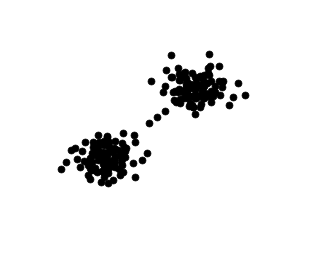
\includegraphics[width=.3\linewidth]{imagenes/c2/TwoBasicsClusters}}
	{
\includegraphics[width=.3\linewidth]{imagenes/c2/MoonsBasics}}
	{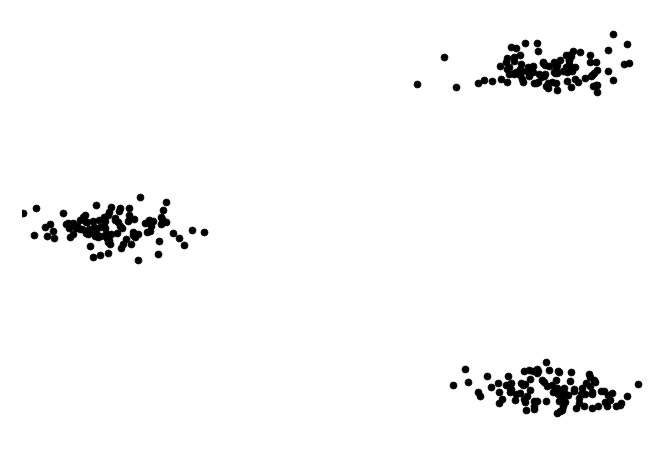
\includegraphics[width=.3\linewidth]{imagenes/c2/ThreeBasicClusters}}
	\caption[Clusters con cohesión interna y/o aislamiento externo]{Clusters con cohesión interna y/o aislamiento externo}\label{fig:figure1}
\end{figure}

Por otra parte, como ya mencionamos anteriormente en esta sección, puede darse el caso de que en un conjunto de datos no exista una partición justificada. En la Figura \ref{fig:figure2} se muestra un conjunto de datos para el que la mayoría de observadores llegaría a la conclusión de que no existen grupos diferenciados, simplemente una nube de puntos uniformemente distribuidos. Idealmente, es de esperar que un método de clustering aplicado a este mismo conjunto de datos llegue a la misma conclusión.

\begin{figure}[!h]
	\centering
	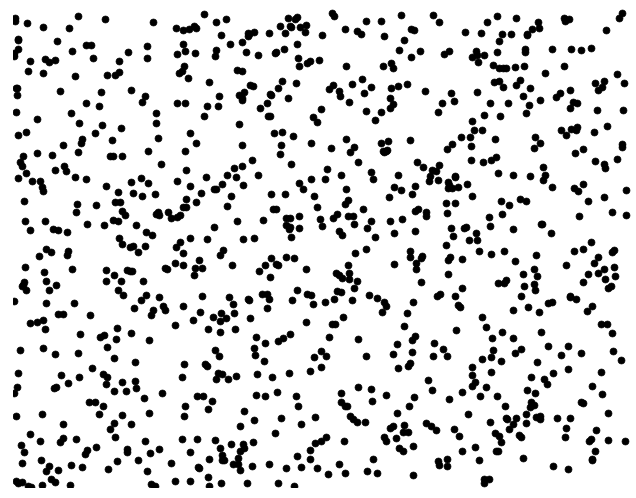
\includegraphics[scale=0.2]{imagenes/c2/rand.png} 
	\caption{Distribución uniforme de puntos}\label{fig:figure2}
\end{figure}

Sin embargo, la mayoría de métodos de aprendizaje no supervisado darán como resultado un particionamiento uniforme como el que se muestra en la Figura \ref{fig:figure3}. El número de particiones encontradas dependerá del método aplicado, si bien en cualquier caso obtendremos un particionamiento uniforme.

\begin{figure}[!h]
	\centering
	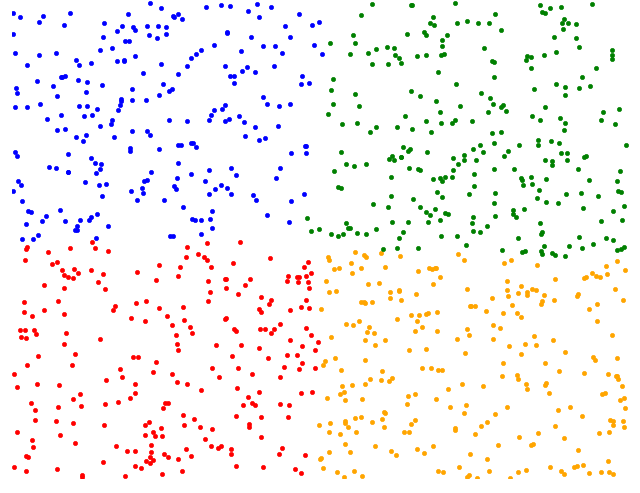
\includegraphics[scale=0.2]{imagenes/c2/randClasif.png} 
	\caption{Distribución uniforme de puntos clasificados}\label{fig:figure3}
\end{figure}

El proceso de dividir una distribución homogénea de datos en diferentes grupos se conoce como disección, y tal proceso puede ser útil en ciertas circunstancias. Sin embargo, dado que en la mayoría de las ocasiones de aplicación real de métodos de clusters, no se conoce a priori la estructura de los datos, existe el riesgo de interpretar todas las soluciones en términos de existencia de subgrupos, lo que conllevaría la imposición de una estructura ficticia en datos en los que no hay estructura presente.

\section{Aplicaciones del clustering}

Como ya se ha indicado, el problema general al que intenta dar solución el clustering está presente en muchas disciplinas: biología, botánica, medicina, psicología, geografía, marketing, procesamiento de imágenes, psiquiatría, arqueología, etc. En esta sección se presentan algunas de las aplicaciones del clustering relacionadas con los citados campos.

\subsection{Aplicaciones en marketing}

Dividir los clientes en grupos homogéneos es una de las tareas más frecuentes en marketing. Un director de marketing podría preguntarse cómo agrupar los posibles clientes según los beneficios potenciales del producto que intenta introducir en el mercado. Por otra parte, un analista de marketing podría estar interesado en agrupar las empresas según sus características financieras, para poder analizarlas y predecir sus estrategias de mercado.

Un ejemplo de aplicación del clustering en este ámbito fue publicado por Green et al. (1967). Así, con un gran número de ciudades disponibles para el análisis, debieron restringir los lugares en los que llevar a cabo sus estudios debido a motivos económicos. Para ello hicieron uso del análisis de clusters, clasificando las ciudades en pequeños grupos basándose en 14 características de las mismas, entre ellas el tamaño e ingresos medios \textit{per capita}. Dado que se esperaba que las ciudades incluidas en un mismo grupo fueran muy similares, escogieron una ciudad de cada uno de ellos para realizar sus estudios.

Otra aplicación del análisis de clusters en el marketing fue descrita por Chakrapani (2004). En este caso, un fabricante de coches cree que comprar un coche deportivo no es una decisión basada sólo en capacidades económicas o edad, sino que es una decisión relacionada con el estilo de vida que llevan aquellos que deciden comprar un coche de estas características, frente a aquellos que no lo hacen. En consecuencia, el fabricante decide realizar un estudio, empleando análisis de clusters, que le permita identificar todas las características relacionadas con las personas que comprarían un coche deportivo, para así enfocar sus campañas de marketing a este sector específicamente.

\subsection{Aplicaciones en astronomía}

Dado un conjunto de datos astronómicos, los investigadores quieren saber, por ejemplo, cuantas clases de estrellas hay presentes en ellos, basándose en algun criterio estadístico. Las preguntas más frecuentes dentro de este ámbito son: ¿Cuantos objetos estadísticamente diferentes están presentes en los datos y a qué clase debe ser asignado cada objeto? ¿Aparecen clases de objetos previamente desconocidas?. El análisis de clusters puede ser aplicado para dar respuesta a estas cuestiones, ayudando a detectar objetos estadísticamente anómalos, así como a guiar el proceso de clasificación de los mismos. Algunos ejemplos incluyen el descubrimiento de quasars con alto corrimiento al rojo, quasars de tipo 2 (altamente luminosos, núcleos galácticos activos a menudo oscurecidos por polvo y gas), y enanas marrones.

Un ejemplo específico viene dado por el estudio de Faúndez-Abans et al. (1996), quienes aplicaron técnicas de clustering a datos sobre la composición química de 192 nebulosas planetarias. Se identificaron 6 grupos diferentes que eran similares en muchos aspectos a una clasificación previa de dichos objetos, pero que también mostraban diferencias interesantes que hasta ese momento los investigadores habían pasado por alto.

Un segundo ejemplo lo encontramos en el estudio de Celeux y Govaert (1992), quienes aplicaron clustering basado en distribuciones normales a un conjunto de 2370 estrellas, descritas por su velocidad relativa al núcleo galáctico y a la rotación galáctica. Usando un modelo de tres clusters, encontraron un cluster de gran tamaño y pequeño volumen, y dos de pequeño tamaño y gran volumen.

\subsection{Aplicaciones en psiquiatría}

Las enfermedades de la mente son a menudo más difíciles de diagnosticar que las enfermedades del cuerpo; es por ello que en el campo de la psiquiatría ha crecido el interés por las técnicas de análisis de clusters que permitan refinar, o incluso redefinir, las técnicas de diagnosis para este tipo de enfermedades. Gran parte de este trabajo involucra pacientes deprimidos, casos en los que el interés reside en distinguir entre dos tipos de depresión, la endógena (congénita), y la neurótica.

Pilowsky et al. (1968), por ejemplo, usando métodos desarrollados por otros autores, aplicaron técnicas de clustering a 200 pacientes en base a sus respuestas a un cuestionario sobre la depresión, junto a información sobre su sexo, edad, estado mental y enfermedad padecida. Éste es un claro ejemplo de variables de diferentes tipos incluidas en el mismo conjunto de datos. Uno de los grupos obtenidos como resultado de este estudio fue identificado como marcador de la depresión endógena.

El análisis de clusters también ha sido empleado para encontrar una clasificación de individuos que intentaron cometer suicidio, que podría sentar las bases para estudios posteriores sobre las causas y tratamientos del problema. Paykey y Rassaby (1978), por ejemplo, estudiaron 236 casos de suicidas fallidos registrados por el servicio de emergencias de una ciudad de los Estados Unidos de América. Del conjunto de posibles variables, 14 fueron seleccionadas como particularmente relevantes para la clasificación y, por tanto, fueron usadas en el análisis. Entre ellas se encontraban: edad, número de intentos de suicidio, gravedad de la depresión y grado de hostilidad, además de una serie de características demográficas. Al conjunto de datos resultante se le aplicó métodos de clustering; el resultado más significativo obtenido corresponde a una división en tres clusters bien definidos.

\subsection{Aplicaciones en meteorología y climatología}

Diariamente se recogen enormes cantidades de datos sobre la meteorología mundial. Explorar estos datos mediante técnicas de clustering puede aportar nuevos enfoques para la climatología y el medio ambiente.

Littmann (2000), por ejemplo, aplicó clustering a los datos recogidos sobre los cambios diarios en la presión superficial en la cuenca Mediterránea, y encontró 20 grupos que explicaban la varianza de las lluvias en las regiones centrales del Mediterráneo. Otro ejemplo viene de la mano de Liu y George (2005), quienes usaron el algoritmo K-medias difuso (\textit{Fuzzy K-means}, \acs{FKM}) con datos espaciotemporales de la climatología de las regiones del sur central de EEUU. 

\subsection{Aplicaciones en arqueología}

La arqueología es otra de las disciplinas en la que resulta útil la aplicación del clustering. La clasificación de los diferentes objetos encontrados en los yacimientos puede ayudar a descubrir su uso, los periodos a los que pertenecen, así como la población que los utilizó. De forma similar, el estudio de materiales fosilizados puede ayudar a revelar como vivieron las sociedades prehistóricas. 

Un ejemplo temprano de la aplicación de clustering a objetos arqueológicos viene dado por Hodson et al. (1966), quienes aplicaron técnicas de clustering a un grupo de broches que datan de la Edad de Hierro, encontrando una clasificación para los mismos de demostrada relevancia arqueológica. Otro ejemplo de la mano de Hodson (1971) es la aplicación del algoritmo K-medias (\acs{KM}, Apéndice \ref{ap:kmeans}) para construir una taxonomía de hachas de mano encontradas en las Islas Británicas. Las variables tenidas en cuenta para describir cada hacha incluyen longitud, anchura y valores en una escala que describen cómo de puntiaguda era la herramienta. El clustering dio como resultado dos grupos de hachas, uno formado por las pequeñas y delgadas, y otro formado por las grandes y gruesas.

Respecto a materiales fosilizados, Sutton y Reinhard (1995) realizaron un estudio sobre 155 coprolitos encontrados en \textit{Antelope House}, un yacimiento prehistórico en el Cañón de Chelly en Arizona. El estudio arrojó como resultado una interpretación de las diferencias entre coprolitos basada en la alimentación.

\subsection{Aplicaciones en bioinformática y genética}

Tiempos recientes están siendo testigo de un tremendo auge en el interés por la Bioinformática, acompañada por la biología molecular, ciencias de la computación, matemáticas y estadística. Tal aumento ha sido acelerado por la siempre creciente base de datos genómica y proteica, que son por sí mismas resultado de un grandísimo avance en las técnicas de secuenciación del ADN, medidas de expresión de los genes y compresión de las estructuras macromoleculares. La estadística ha resultado relevante en el estudio de la expresión de los genes. Los genes contenidos en el ADN de cada célula proporcionan las plantillas necesarias para la generación de las proteínas implicadas en la mayoría de los procesos estructurales y biomecánicos que tienen lugar en cada uno de nosotros. Sin embargo, aunque la mayoría de las células en los seres humanos contienen todos los complementos genéticos que componen el genoma humano, los genes se expresan de manera selectiva en cada célula dependiendo del tipo de la misma, del tejido y de las condiciones generales tanto dentro como fuera de la célula. La biología molecular ha puesto de manifiesto que la mayoría de los procesos en la vida de una célula están regulados por factores que afectan a la expresión de sus genes.

Como hemos visto, uno de los campos de investigación más activos hoy en día es el que estudia los procesos que regulan la expresión de los genes. Con el fin de almacenar la información relativa a esta área de estudio surgen los microarrays, (Cortesse, 2000). Desde el punto de vista del análisis de datos, una de las características relevantes en este tipo de información es que el número de atributos de cada instancia ($p$), supera con creces al número de instancias disponibles ($n$); conjuntos de datos como este son calificados como \textit{datos de alta dimensionalidad}.

La mayoría de métodos estadísticos clásicos no pueden ser aplicados a este tipo de conjuntos de datos sin ser modificados de forma sustancial. Sin embargo, el análisis de clusters acepta bien tales conjuntos de datos y puede ser empleado para identificar grupos de genes con patrones de expresión similares, y dar respuesta a preguntas como por qué un gen se ve afectado por cierta enfermedad, o qué genes son responsables de enfermedades genéticas hereditarias.

Un ejemplo de aplicación lo encontramos en el trabajo de Selinski e Ickstadt (2008), quienes usaron clustering sobre polimorfismos de nucleótidos simples para detectar diferencias entre enfermedades a nivel genético.

\section{Resumen}

El clustering consiste en la exploración de conjuntos de datos. Su objetivo es discernir si pueden o no ser resumidos de manera significativa, en términos de un número relativamente pequeño de grupos o clusters de objetos o individuos, que se parecen unos a otros y que se diferencian de los que se encuentran en otros clusters.

Muchas ramas de la ciencia han hecho uso de las técnicas de clustering de manera exitosa, para avanzar en sus respectivos campos, y procesar grandes cantidades de datos, cuyo análisis sería impensable afrontar con técnicas tradicionales.

%Para referir un acronimo completo \acf
%Para referir un acronimo solo con las siglas \acs





















\chapter{Clustering con restricciones}\label{ch:Clustering con restricciones}

Realizada la introducción sobre los conceptos básicos del clustering, el objetivo de este capítulo es definir los conceptos relacionados con el clustering con restricciones, así como dar ejemplos de su aplicación y destacar los beneficios y problemas que presenta su uso. A tal fin tomamos como referencia principal el trabajo de Ian Davidson y Sugato Basu (2007) \cite{Survey:2007} entre otros.

\section{Motivación para el clustering con restricciones}

Tal y como hemos estudiado en el Capítulo \ref{ch:Breve introducción al Clustering}, los métodos de clustering no supervisado son útiles para dotar de estructura a datos referentes a un área concreta. Un ejemplo de ello lo encontramos en la clasificación de textos; Cohn et al. (2003) \cite{Cohn:2003} afrontan un problema propuesto por Yahoo!, que consiste en, dada una gran cantidad de documentos de texto, agruparlos según una taxonomía en la que los documentos con temáticas similares se encuentren cercanos. Para ello, los métodos de clustering no supervisado resultan de utilidad, ya que la información sobre el problema de la que se dispone inicialmente es limitada. Sin embargo, Wagstaff et al. (2001) mostraron que aplicando clustering no supervisado a ciertos problemas, como el de agrupar datos de GPS de forma que los clusters definan los carriles de una vía, no se obtienen resultados significativos, pues los clusters obtenidos distan mucho de la forma alargada que se esperaría como resultado. Para atajar el problema, introdujeron en el clustering un nuevo elemento, las restricciones a nivel de instancia, que permitían incluir conocimiento sobre los clusters que guiarían los métodos de clustering para obtener los resultados esperados. Bastaba con indicar que los carriles de la vía por la que circulan los vehículos miden cuatro metros de ancho, y por tanto cualquier vehículo que se encuentre a una distancia mayor de 4 metros de otro, en dirección perpendicular a la del desplazamiento, debe ser ubicado en un cluster diferente.

Nos situamos entonces en un nuevo escenario: es posible incorporar información adicional al proceso de clustering, además de la contenida en el propio conjunto de datos, para guiarlo en la formación de la partición y obtener resultados más precisos. Esto sitúa al clustering con restricciones en el marco del aprendizaje semisupervisado, a diferencia de los métodos de clustering tradicionales que se enmarcan en el área del clustering no supervisado. 

\section{Definición de las restricciones}

El nuevo tipo de  información que incorporamos al clustering viene dado en forma de restricciones a nivel de instancia, esto es, especificar si dos instancias del conjunto de datos deben estar en el mismo cluster o, por el contrario, deben estar en clusters separados.

A las restricciones que indican que dos puntos deben ser situados en el mismo cluster se las denomina \textit{Must-link}, y se notan con $ML(x,y)$, donde $x$ e $y$ son dos instancias del conjunto de datos. De manera similar, a las restricciones que especifican lo contrario se las denomina \textit{Cannot-link}, y se notan con $CL(x,y)$. \cite{WagstaffCardie:2000}

Aunque pueden parecer simples, las restricciones definidas de la anterior forma poseen propiedades interesantes. Las Restricciones de tipo Must-link son un ejemplo de relación de equivalencia, y por tanto son simétricas, reflexivas y transitivas, formalizando:

\begin{observacion}
	\textbf{Las restricciones de tipo ML son transitivas.} Sean $CC_i$ y $CC_j$ componentes conexas, conectadas mediante restricciones $ML$, y sean $x$ e $y$ dos instancias en $CC_i$ y $CC_j$ respectivamente. Entonces $ML(x,y): x \in CC_i, y \in CC_j \rightarrow ML(a,b) \forall a,b: a\in CC_i, b \in CC_j$. \cite{Survey:2007}
\end{observacion}

\begin{observacion}
	\textbf{Las restricciones de tipo CL pueden ser deducidas.} Sean $CC_i$ y $CC_j$ componentes conexas, conectadas mediante restricciones $ML$, y sean $x$ e $y$ dos instancias en $CC_i$ y $CC_j$ respectivamente. Entonces $CL(x,y): x \in CC_i, y \in CC_j \rightarrow CL(a,b) \forall a,b: a\in CC_i, b \in CC_j$. \cite{Survey:2007}
\end{observacion}

Un claro ejemplo de uso de las restricciones lo encontramos en casos de aplicación de clustering en los que existen limitaciones en cuanto a las medidas de distancia, como sucedía en el supuesto de los datos GPS. Así, si queremos que las instancias que forman dos clusters estén separadas por una distancia mayor o igual a $\delta$, basta con establecer restricciones de tipo ML entre todas aquellas instancias cuya distancia sea menor que $\delta$. 
De manera similar, si queremos que el diámetro de los clusters sea como mucho $\epsilon$, debemos establecer un conjunto de restricciones de tipo CL entre todas aquellas instancias que se encuentren a una distancia mayor que $\epsilon$. La Figura \ref{fig:figure4} muestra una representación gráfica de estos dos tipos de restricciones.

\begin{figure}[!h]
	\centering
	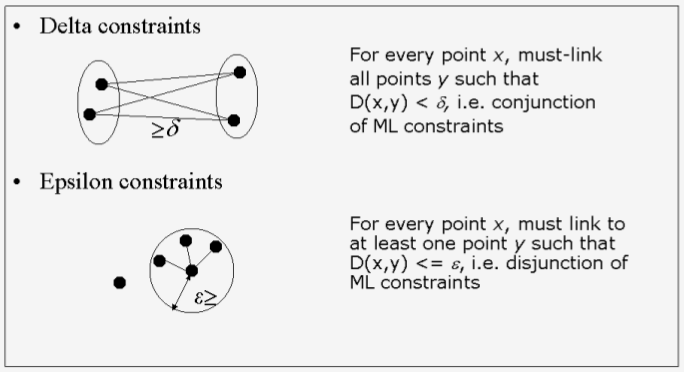
\includegraphics[scale=0.45]{imagenes/c3/RestriccionesDeltaEpsilo.png} 
	\caption[Restricciones de tipo \textit{delta} y \textit{épsilon}.]{Restricciones de tipo \textit{delta} y \textit{épsilon}. \cite{Survey:2007}}\label{fig:figure4}
\end{figure}


\section{Uso de las restricciones}

Mientras que el aprendizaje completamente supervisado implica conocer la etiqueta asociada a cada instancia, en el aprendizaje semisupervisado sólo se dispone de un subconjunto de instancias etiquetadas. Por otra parte, en gran cantidad de dominios la información disponible se refiere a relaciones entre instancias, y no a la clase concreta a la que pertenecen las mismas. Es más, en sistemas de clustering interactivo, un usuario no experto en el dominio del problema podrá, probablemente, aportar información en forma de restricciones de tipo \acf{ML} y \acf{CL} \cite{Cohn:2003}\cite{DavidsonRavi:2007}, antes que aportar información sobre a qué clase concreta pertenecen ciertas instancias.

Habitualmente, las restricciones se incluyen en los problemas de clustering de dos maneras. Pueden ser empleadas para modificar la regla de asignación de instancias a clusters del método en cuestión, de forma que la solución satisfaga el máximo número de restricciones posible. Alternativamente, cabe la posibilidad de entrenar la función de distancia empleada por el método en base a las restricciones, ya sea antes o durante la aplicación del mismo. En cualquier caso, la fase de inicialización puede tomar en consideración las restricciones, de forma que las instancias asociadas con restricciones \acf{ML} serán situadas en el mismo cluster, y aquellas entre las que exista una restricción \acf{CL}, quedarán en clusters diferentes. Basándonos en esta distinción, identificamos dos maneras de aproximar el problema, las basadas en restricciones (\textit{constraint-based}), y las basadas en distancias (\textit{distance-based}).

\subsection{Métodos basados en restricciones}

En los métodos basados en restricciones, el propio método de clustering es modificado de manera que la información disponible se emplea para sesgar la búsqueda y obtener una partición de los datos apropiada.

Existen dos modelos de métodos basados en restricciones: (1) aquellos que fuerzan el cumplimiento de las restricciones, e intentan encontrar la mejor asignación posible que no infrinja ninguna de ellas \cite{Wagstaff:2001b}\cite{DavidsonRavi:2005b}, y (2) los que hacen una interpretación relajada de las restricciones \cite{Basu:2004}\cite{Seagal:2003}\cite{DavidsonRavi:2005a}\cite{Law:2005}, permitiéndose incumplir un número mínimo de ellas para optimizar la función objetivo; de esta manera surge un compromiso entre el número de restricciones incumplidas y el valor de la función objetivo. Existen diversas técnicas para obtener una partición atendiendo a las restricciones:

\begin{itemize}
	
	\item Modificar la función objetivo de manera que incluya una penalización por incumplir restricciones. \cite{Demiriz:1999} \cite{DavidsonRavi:2005a}
	
	\item Agrupar instancias con información adicional obtenida de una distribución condicional en un espacio auxiliar. \cite{SinkkonenKaski:2000}
	
	\item Forzar el cumplimiento de todas las restricciones modificando la regla de asignación del método. \cite{Wagstaff:2001b}
	
	\item Inicializar los clusters en base a restricciones inferidas del conjunto de instancias etiquetadas.\cite{Basu:2002}
	
\end{itemize}

La Figura \ref{fig:figure5} muestra un conjunto de datos junto a sus restricciones asociadas. La Figura \ref{fig:figure6} propone un posible agrupamiento que satisface todas las restricciones.

\begin{figure}[bth]
	\myfloatalign
	{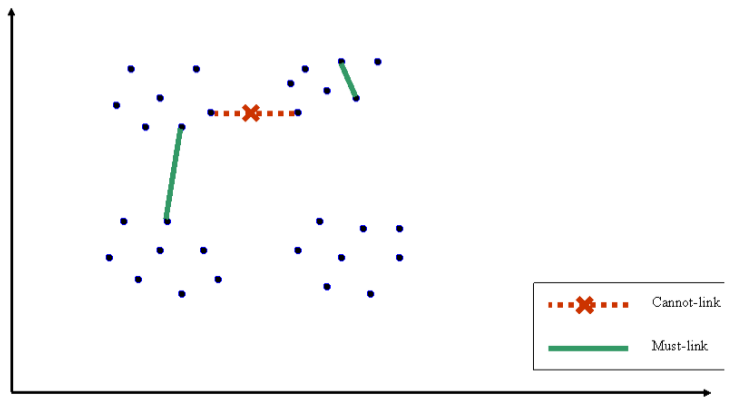
\includegraphics[width=.6\linewidth]{imagenes/c3/InputInstancesAndConst1}
	\caption[Restricciones sobre un conjunto de datos.]{Restricciones sobre un conjunto de datos. \cite{Survey:2007}} \label{fig:figure5}
	}
	{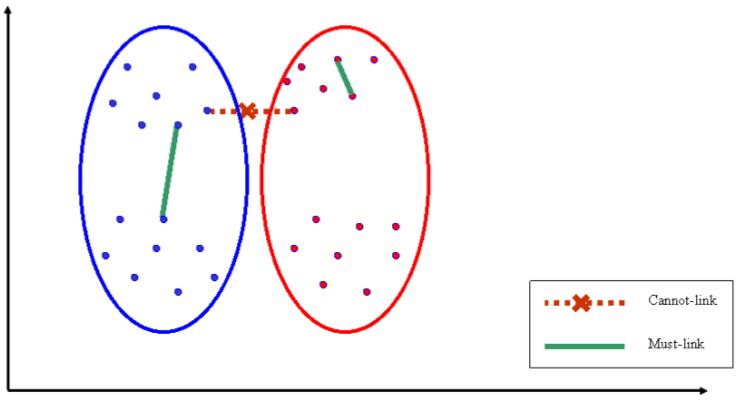
\includegraphics[width=.6\linewidth]{imagenes/c3/ClusteringSatAll}
	\caption[Clustering que satisface todas las restricciones.]{Clustering que satisface todas las restricciones. \cite{Survey:2007}} \label{fig:figure6}
	}
\end{figure}

\subsection{Métodos basados en distancia}

En las aproximaciones basadas en distancias se emplean métodos de clustering clásicos que hacen uso de una medida de distancia, de forma que dicha medida se modifica para que tenga en consideración las restricciones. En este contexto, satisfacer las restricciones significa que las instancias relacionadas con restricciones \acf{ML} se sitúan juntas en el espacio, y las relacionadas mediante \acf{CL} se encuentran separadas.

La Figura \ref{fig:figure8} muestra un posible agrupamiento basado en una métrica aprendida a partir de las restricciones especificadas en la Figura \ref{fig:figure7}. Cabe destacar que en la Figura \ref{fig:figure8} el espacio en el que se encuentran los datos ha sido comprimido en el eje vertical y ensanchado en el eje horizontal para ajustarlo a la métrica de distancia aprendida.

\begin{figure}[bth]
	\myfloatalign
	{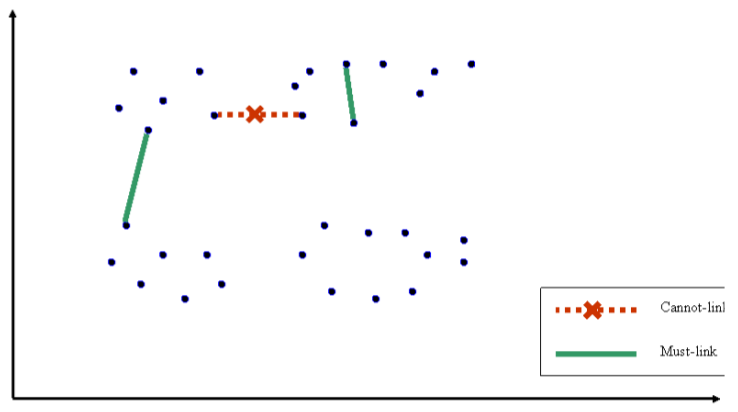
\includegraphics[width=.6\linewidth]{imagenes/c3/InputInstancesAndConst2}
	\caption[Restricciones sobre un conjunto de datos.]{Restricciones sobre un conjunto de datos. \cite{Survey:2007}} \label{fig:figure7}
	}
	{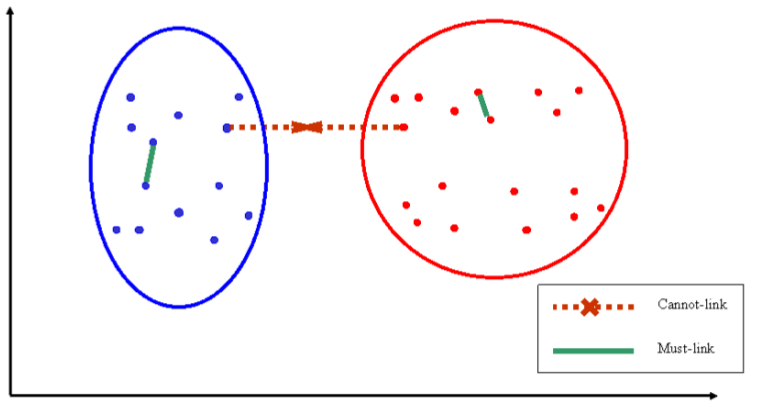
\includegraphics[width=.6\linewidth]{imagenes/c3/MetricaAprendida}
	\caption[Clustering basado en métrica aprendida en base a las restricciones.]{Clustering basado en métrica aprendida en base a las restricciones. \cite{Survey:2007}} \label{fig:figure8}
	}
\end{figure}

\section{Aplicaciones del clustering con restricciones} \label{aplicacion}

Esta sección muestra algunos casos de aplicación en los que el clustering con restricciones ha resultado ser una herramienta más útil que el clustering no supervisado. Para cada caso analizaremos cómo se obtuvieron las restricciones y cómo éstas mejoran los resultados en el clustering resultante. 

\subsection{Aplicaciones en análisis de imágenes}

La Figura \ref{fig:figure9} muestra un extracto del conjunto de datos de caras de  CMU (Carnegie Mellon University), en el que la tarea es agrupar caras en base a diferentes criterios. En este caso, el objetivo es agrupar las caras según su orientación.

\clearpage

\begin{figure}[bth]
	\myfloatalign
	\subfloat[Caras de perfil]
	{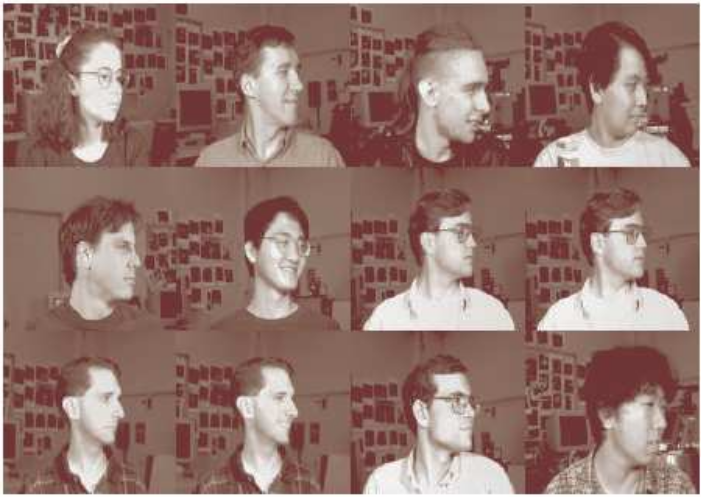
\includegraphics[width=.3\linewidth]{imagenes/c3/AnalisisImagenes/Caras1}} \quad
	\subfloat[Caras de frente.]
	{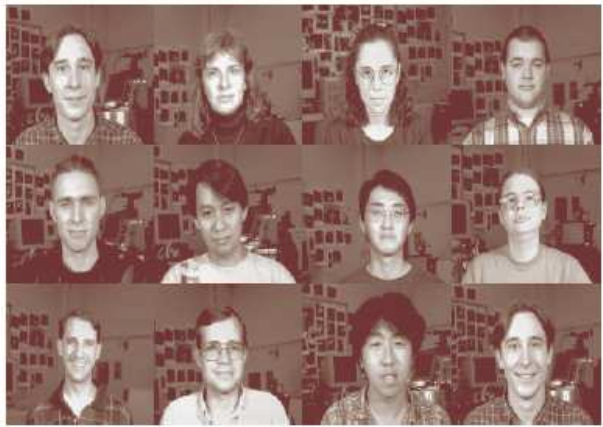
\includegraphics[width=.3\linewidth]{imagenes/c3/AnalisisImagenes/Caras3}} \quad
	\subfloat[Caras hacia arriba.]
	{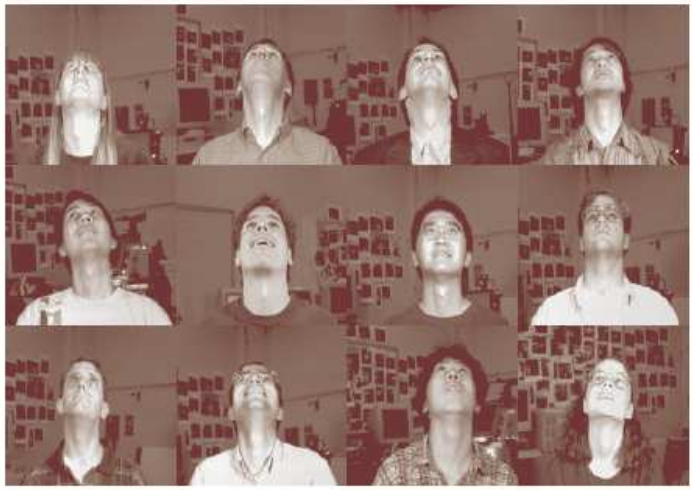
\includegraphics[width=.3\linewidth]{imagenes/c3/AnalisisImagenes/Caras2}} \quad
	\caption[Caras de la base de datos de  CMU.]{Caras de la base de datos de  CMU. \cite{Survey:2007}}\label{fig:figure9}
\end{figure}

El método empleado para extraer las restricciones es uno de los más populares en la literatura: establecer el número de clusters de la partición resultado igual al número de clases en la base de datos, y generar las restricciones a partir de un subconjunto de instancias etiquetadas; esto es, si dos instancias tiene diferentes etiquetas, establecer una restricción \acf{CL} entre ellas, en caso contrario una de tipo \acf{ML}. De esta forma, entre las imágenes mostradas en la Figura \ref{fig:figure10} se establecen restricciones \acf{CL}, ya que, aunque pertenecen a la misma persona, no presentan la misma orientación.

\begin{figure}[bth]
	\myfloatalign
	{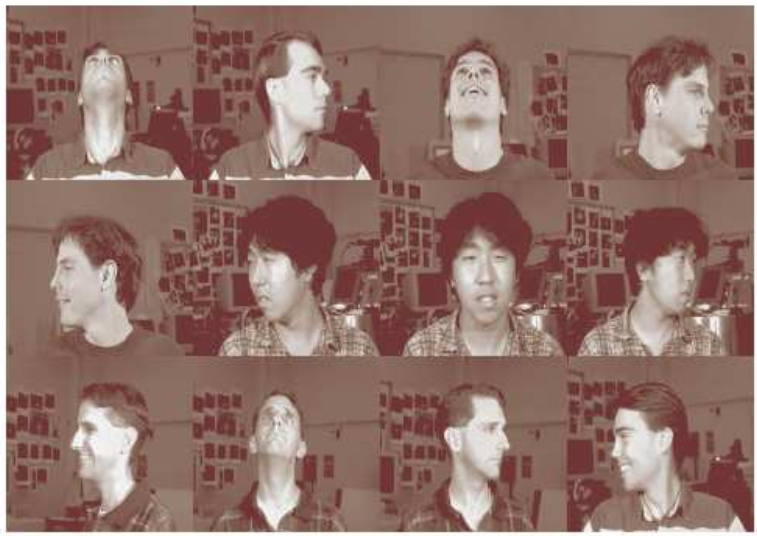
\includegraphics[width=.35\linewidth]{imagenes/c3/AnalisisImagenes/CarasDifOr1}} \quad
	{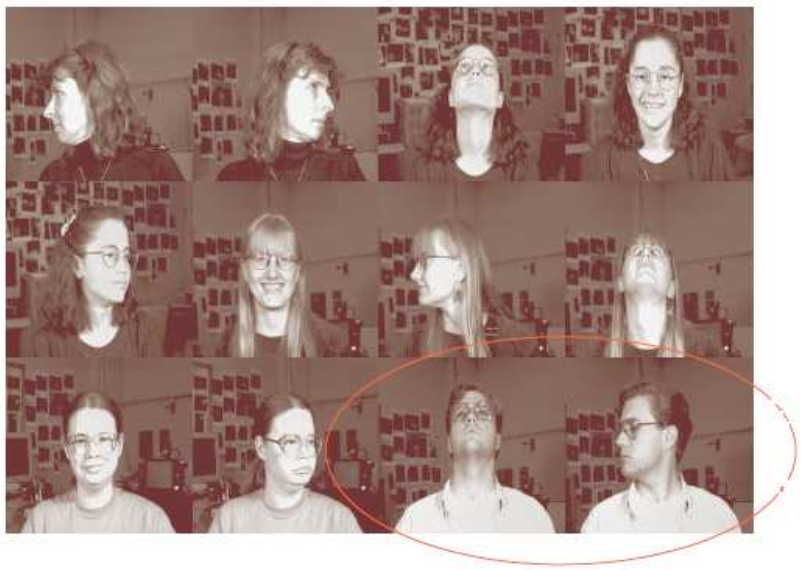
\includegraphics[width=.35\linewidth]{imagenes/c3/AnalisisImagenes/CarasDifOr2}}
	\caption[Restricciones de tipo \ac{CL} entre caras de la misma persona.]{Restricciones de tipo \ac{CL} entre caras de la misma persona.  \cite{Survey:2007}}\label{fig:figure10}
\end{figure}

En la Figura \ref{fig:figure11} se muestra otro conjunto de datos de imágenes sobre el que se aplican técnicas de clustering con restricciones. En este caso, la tarea es realizar reconocimiento de objetos para incorporar el método al sistema de navegación del robot Aibo \cite{DavidsonRavi:2005a}. Para ello se emplean restricciones de distancia de tipo $\delta$ y $\epsilon$ como las descritas en la Figura \ref{fig:figure4}. De esta manera se consiguen clusters bien diferenciados y por tanto útiles para las tareas de búsqueda de caminos que el robot realiza durante la navegación.

\begin{figure}[bth]
	\myfloatalign
	\subfloat[Imagen original]
	{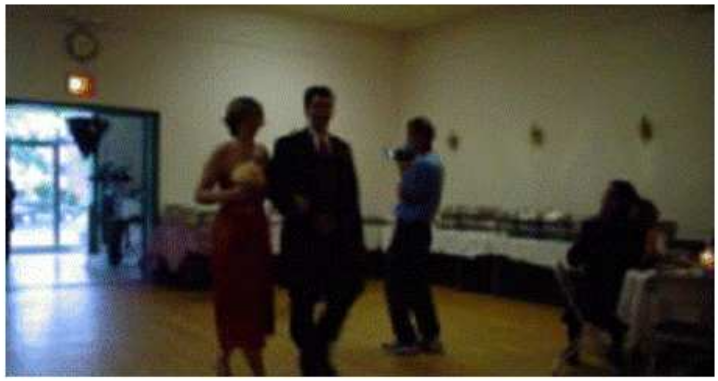
\includegraphics[width=.3\linewidth]{imagenes/c3/AnalisisImagenes/Aibo1}} \quad
	\subfloat[Clustering sin restricciones]
	{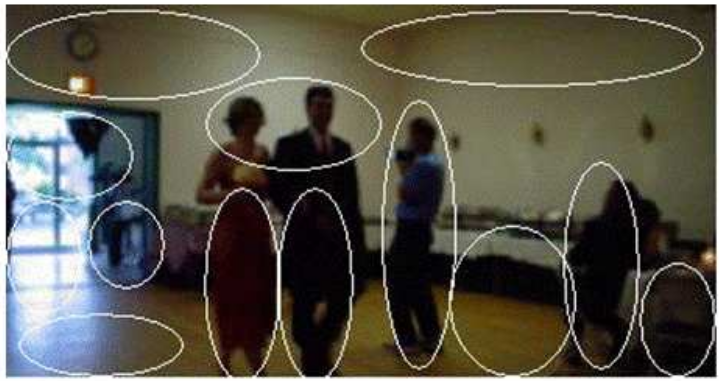
\includegraphics[width=.3\linewidth]{imagenes/c3/AnalisisImagenes/Aibo2}} \quad
	\subfloat[Clustering con restricciones]
	{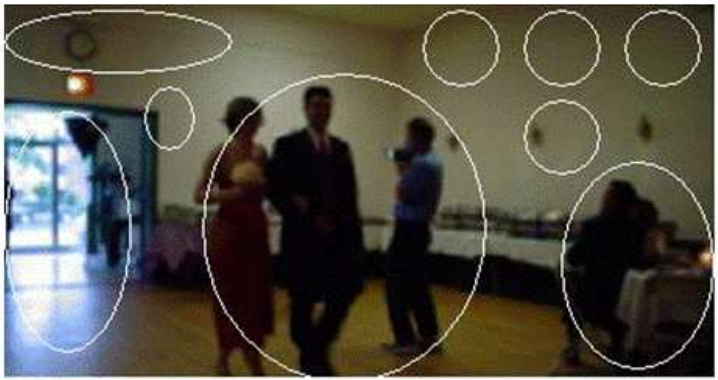
\includegraphics[width=.3\linewidth]{imagenes/c3/AnalisisImagenes/Aibo3}} \quad
	\caption[Método de clustering empleado en el sistema de navegación del robot Aibo.]{Método de clustering empleado en el sistema de navegación del robot Aibo. \cite{Survey:2007}\cite{DavidsonRavi:2005a}}\label{fig:figure11}
\end{figure}

\subsection{Aplicaciones en análisis de vídeos}

Las bases de datos de vídeo son uno de los ejemplos en los que las restricciones pueden ser generadas directamente desde el dominio de datos, especialmente disponiendo de datos espacio-temporales sobre el vídeo \cite{Yan:2006}. En datos temporalmente sucesivos es posible establecer restricciones de tipo \acf{ML} entre grupos de píxeles de fotogramas (\textit{frames}) cercanos en el tiempo. Esto es especialmente útil cuando la tarea es implementar reconocimiento de objetos basado en clustering y segmentación. También es posible añadir restricciones \acf{CL} a clusters localizados en el mismo fotograma, ya que existe una baja probabilidad de que estén asociados al mismo objeto. De hecho, en el dominio asociado a problemas de análisis de vídeo existen gran variedad de métodos de extracción de restricciones \cite{Yan:2006}, la Figura \ref{fig:figure12} muestra algunos ejemplos.  

\begin{figure}[bth]
	\myfloatalign
	\subfloat[]
	{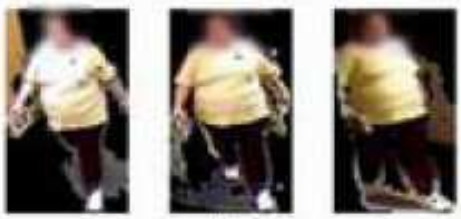
\includegraphics[width=.4\linewidth]{imagenes/c3/Videos/VideoA}}
	\quad
	\subfloat[]
	{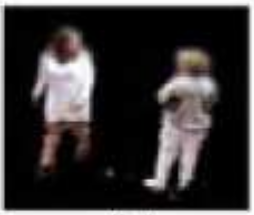
\includegraphics[width=.225\linewidth]{imagenes/c3/Videos/VideoB}} \quad
	\subfloat[]
	{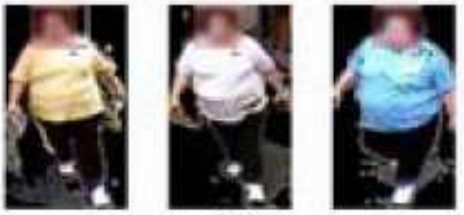
\includegraphics[width=.4\linewidth]{imagenes/c3/Videos/VideoC}}
	\quad
	\subfloat[]
	{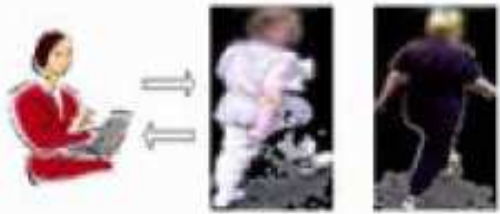
\includegraphics[width=.4\linewidth]{imagenes/c3/Videos/VideoD}}
	\caption[Diferentes tipos de restricciones en datos de video.]{Diferentes tipos de restricciones en datos de video. \cite{Yan:2006} \cite{Survey:2007}}\label{fig:figure12}
\end{figure}

En la Figura \ref{fig:figure12}, la imagen (a) corresponde a restricciones extraídas del seguimiento de una persona durante un periodo de tiempo, la (b) corresponde a restricciones espaciales que asocian dos objetos localizados en el mismo fotograma, la imagen (c) corresponde a restricciones obtenidas mediante reconocimiento facial y la (d) a las proporcionadas por el usuario.

Disponiendo de tantos métodos para extraer restricciones, cabe plantearse: ¿qué sucede si se establecen demasiadas restricciones? ¿Hace esto que el problema esté sobrerestringido? En la Sección \ref{Problemas} abordaremos estas cuestiones.

\subsection{Aplicaciones en genética}

En clustering de genes basado en microarrays, los genes vienen representados por su perfil de expresión en diferentes experimentos y agrupados empleando diferentes métodos, en este caso métodos de clustering con restricciones. La  Figura \ref{fig:figure13} muestra un ejemplo: se trata de restricciones de tipo \acf{ML} que se establecen entre genes en base a los datos de co-ocurrencia almacenados en la base de datos de interacciones de proteínas, que contiene información sobre qué genes (y sus proteínas asociadas) están presentes en los mismos procesos celulares \cite{Xenarios:2001}. Esta información puede ser empleada para mejorar los resultados que proporcionan los métodos de clustering. \cite{Seagal:2003}

\begin{figure}[!h]
	\centering
	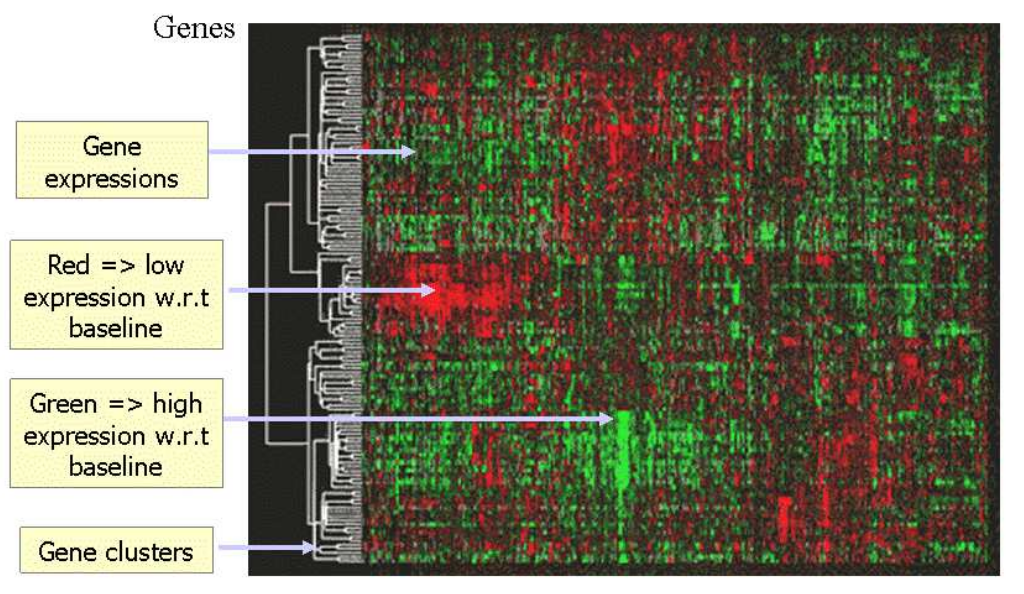
\includegraphics[scale=0.3]{imagenes/c3/Genetica/Genes} 
	\caption[Clustering de genes basado en microarrays.]{Clustering de genes basado en microarrays. \cite{Survey:2007}}\label{fig:figure13}
\end{figure}

\subsection{Aplicaciones en análisis de textos}

En tareas de clasificación de contenido, el objetivo es dividir de manera automática grandes cantidades de documentos en grupos o clusters. En este caso es posible extraer las restricciones de múltiples recursos auxiliares. Por ejemplo, si dos documentos se encuentran en el mismo directorio se podría inferir una restricción de tipo \acf{ML} entre ellos. De esta manera es posible modificar el clustering resultante para que se adapte a un criterio concreto, como por ejemplo crear una jerarquía de documentos semejante a la forma en la que se encuentran organizados en la estructura de directorios de entrada.

\subsection{Aplicaciones en datos web} 

El clustering con restricciones resulta de gran utilidad en el procesamiento de datos de búsqueda en páginas web. Aquí, el objetivo es agrupar, de manera automática, los resultados de una consulta ambigua en el motor de búsqueda en clusters de \acs{URL}s, que se refieran al concepto introducido como consulta en diferentes contextos. En este ámbito es posible extraer las restricciones a partir de búsquedas realizadas anteriormente por los usuarios, de manera que se establece una restricción de tipo \acf{ML} entre \acs{URL}s visitadas en la misma sesión de usuario. Aplicar clustering utilizando estas restricciones puede ayudar a sesgar el resultado de las búsquedas hacia las preferencias del usuario.

\subsection{Aplicaciones en datos de audio}

En ciertas tareas de análisis de audio, es posible que no se conozca el número de clases de objetos presentes en los datos, si bien las restricciones pueden extraerse directamente del dominio de datos. Esto sucede, por ejemplo, al aplicar clustering para reconocimiento de hablantes en una conversación \cite{BarHillel:2003}. En este caso el número de participantes no se conoce a priori, pero es fácil detectar si dos hablantes son diferentes o similares y establecer las restricciones en base a ello.

\subsection{Aplicaciones en datos de GPS} \label{EjemploGPS}

Tal y como se indicó en el inicio del Capítulo \ref{ch:Clustering con restricciones}, el clustering con restricciones sobre datos \acs{GPS} se utiliza para identificar el carril por el que circula cada vehículo, como se muestra en la Figura \ref{fig:figure14}. Cada instancia viene representada por la posición que ocupa en la vía en coordenadas cartesianas bidimensionales $(x,y)$, obtenidas en base a los datos \acs{GPS}. La Figura \ref{fig:figure15} muestra de manera gráfica esta representación de los datos (cabe destacar que múltiples instancias pueden referirse al mismo vehículo en distintos momentos en el tiempo).

\begin{figure}[!h]
	\centering
	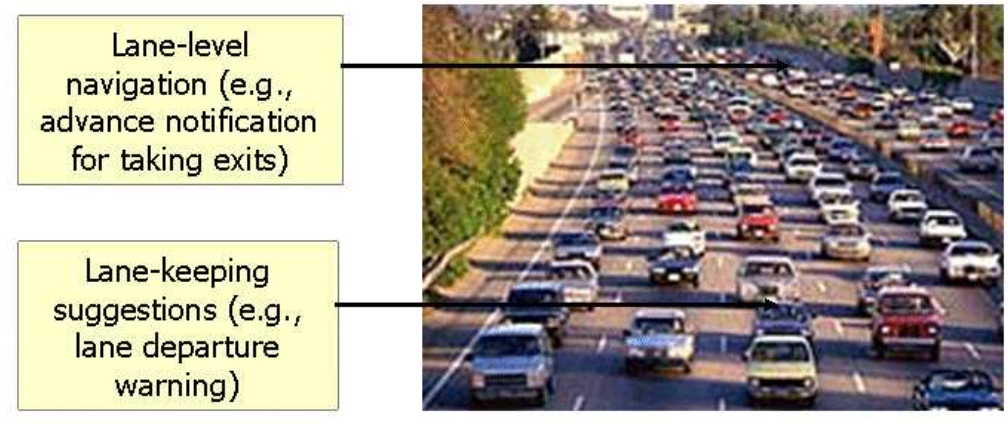
\includegraphics[scale=0.3]{imagenes/c3/GPS/Coches} 
	\caption[Uso de información GPS.]{Uso de información GPS. \cite{Survey:2007} \cite{Wagstaff:2001b}}\label{fig:figure14}
\end{figure}


En este dominio, los clusters reales tiene forma alargada en el eje horizontal y se encuentran alineados perpendicularmente a la dirección de desplazamiento. Para lograr que los clusters resultantes tengan esta forma, podemos hacer uso de las restricciones. Estableceremos una restricción de tipo \acf{CL} entre aquellas instancias separadas más de 4 metros en dirección perpendicular a la del desplazamiento (ya que los carriles tiene una anchura máxima de 4 metros), y \acf{ML} entre aquellas instancias que presenten continuidad en el eje horizontal, puesto que es probable que los vehículos que representan se encuentren en el mismo carril. Este modelo de clustering ha probado ser muy útil en navegación en tiempo real \cite{Wagstaff:2001b}, permitiendo notificar al usuario cuando debe cambiar de carril, o cuando no debe abandonarlo.

\begin{figure}[!h]
	\centering
	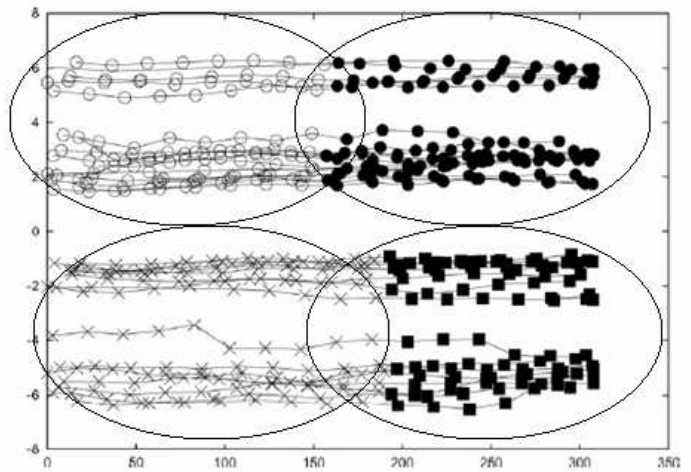
\includegraphics[scale=0.32]{imagenes/c3/GPS/Instancias} 
	\caption[Clusters encontrados en datos GPS sin uso de restricciones.]{Clusters encontrados en datos \acs{GPS} sin uso de restricciones. \cite{Survey:2007} \cite{Wagstaff:2001b}}\label{fig:figure15}
\end{figure}

\section{Beneficios del uso de restricciones}

Encontramos dos beneficios principales en el uso de restricciones: 

\begin{itemize}
	
	\item Incremento de la exactitud en las predicciones de las etiquetas al generar restricciones en base a un subconjunto de instancias etiquetadas.
	
	\item Obtención de clusters con geometría adaptable a cada problema.
	
\end{itemize}

A continuación se analizan estos dos beneficios:

Dado $X = \{x_1 \cdots x_u\}$, un gran conjunto de instancias no etiquetadas, y $L = \{(x_{u+1}, y_{u+1})\cdots (x_{u+l}, y_{u+l})\}$, un pequeño conjunto de instancias etiquetadas, es común escoger dos elementos de $L$ (con reemplazamiento) y establecer una restricción \acs{ML} entre ellos si pertenecen a la misma clase o, en caso contrario, una de tipo \acs{CL}. Un método apropiado para evaluar los resultados ofrecidos por un método de clustering es medir el nivel de exactitud de éste a la hora de predecir las etiquetas del conjunto $X$. Esto normalmente requiere que se especifique el número de clusters deseados igual al número de clases conocidas en $X$ ($K = K^*$). Para medir la exactitud se emplean métodos como \textit{Rand Index} \cite{Rand:1971}.

El trabajo de Wagstaff y Cardie \cite{WagstaffCardie:2000}, en el que generaban las restricciones de la manera descrita anteriormente, demostraba que, cuando se realiza un promedio de la exactitud de las predicciones obtenidas con algoritmos de clustering con restricciones, variando estas últimas entre experimentos, se obtienen resultados hasta un 20\% mejores que con las técnicas clásicas.

\begin{observacion}
	
	\textbf{El uso de restricciones, en promedio, incrementa la precisión.}
	El rendimiento de un método al predecir etiquetas aumenta cuando se promedia empleando numerosos conjuntos de restricciones diferentes. \cite{Survey:2007}
	\label{ob:observacion33}
	
\end{observacion}

Esta regla, sin embargo, no es cierta en todos los casos, pues en conjuntos de datos como \textit{Tic-Tac-Toe Endgame}, no se consigue ningún incremento en las predicciones sea cual sea el número de restricciones empleadas. La explicación dada por los autores citados para estas excepciones se basa en que establecer $K = K^*$ no es apropiado en este caso.

El otro beneficio que reporta el uso de restricciones es la posibilidad de obtener clusters con la geometría deseada, como el ejemplo de aplicar clustering a datos \acs{GPS}, analizado en la Sección \ref{EjemploGPS} de este trabajo.

\section{Problemas del uso de restricciones} \label{Problemas}

Aunque, tal y como hemos comprobado, la incorporación de restricciones a los métodos de clustering reporta beneficios en algunas aplicaciones, existen dos inconvenientes principales que se exponen a continuación, así como posibles soluciones a los mismos.

\subsection{El problema de la factibilidad}

La introducción de restricciones en el clustering cambia el problema al que éste da solución, que pasa a ser: \textit{Encontrar la mejor partición que satisfaga todas las restricciones}. De esta manera, si aquellas no están bien especificadas o si los métodos de extracción son inadecuados, podemos encontrar que las restricciones se contradicen, lo que deriva en que no existe una asignación de instancias a clusters que las satisfaga todas. Por ejemplo, no existe asignación que satisfaga las restricciones $ML(x_1,x_2)$ y $CL(x_1,x_2)$, independientemente del valor de $K$. Lo mismo sucede para $K = 2$, y las restricciones $CL(x_1, x_2)$, $CL(x_2, x_3)$ y $CL(x_1, x_3)$. Formalizando, el problema de la factibilidad para problemas de clustering (no jerárquico) con restricciones viene definido por:

\begin{definicion}
	
	\textbf{Problema de la factibilidad para clustering con restricciones:} Dado un conjunto de datos $X$, un conjunto de restricciones $R$, un umbral superior $K_l$ y un umbral superior $K_u$ para el número de clusters resultantes, ¿Existe una partición de $X$ en bloques tal que $K_l \le K \le K_u$ y todas las restricciones en $R$ se satisfacen? \cite{DavidsonRavi:2005a} \cite{Survey:2007}
	
\end{definicion}

La complejidad teórica del problema dependerá del tipo de restricciones que se combinen en él. La Tabla \ref{tab:tabla1} presenta, de manera resumida, la complejidad esperada en cada caso. 

\begin{table}[h]
	\centering
	\setlength{\arrayrulewidth}{1mm}
	\setlength{\tabcolsep}{10pt}
	\renewcommand{\arraystretch}{1}
	
	\rowcolors{2}{gray!25}{white}
	\begin{tabular}{ >{\centering\arraybackslash}m{4cm}  >{\centering\arraybackslash}m{4cm} }
		\hline
		\rowcolor{black}
		\multicolumn{2}{c}{\bf \color{white}{Complejidad del clustering con restricciones}}\\
		\hline
		\rowcolor{gray!50}
		\textbf{Restricciones} & \textbf{Complejidad} \\
		Restricciones $\delta$ & $\mathbf{P}$ \\
		Restricciones $\epsilon$ & $\mathbf{P}$ \\
		\acs{ML} y $\delta$ & $\mathbf{P}$ \\
		\acs{ML} y $\epsilon$ & $\mathbf{NP}$-completo \\
		$\epsilon$ y $\delta$ & $\mathbf{P}$ \\
		\acs{CL} y otra & $\mathbf{NP}$-completo \\
		\hline
		
	\end{tabular}
	\caption[Complejidad del problema del clustering en función del tipo de restricciones]{Complejidad del problema del clustering en función del tipo de restricciones. \cite{Survey:2007}}
	\label{tab:tabla1}
\end{table}

Tal y como queda reflejado en la Tabla \ref{tab:tabla1}, la utilización de restricciones \acf{CL} eleva el nivel de complejidad del clustering a $\mathbf{NP}$-completo y, por tanto, el problema del clustering con restricciones es intratable. De manera intuitiva puede entenderse fácilmente que, si encontrar una sola partición que satisfaga las restricciones es un problema complejo, más complejo es aún encontrar la mejor. 

\begin{observacion}
	
	\textbf{Saber que existe una solución factible no nos ayuda a encontrarla.} Las consecuencias de este resultado sobre la complejidad del clustering con restricciones implican que, aun en caso de que exista una partición factible, no será fácil de encontrar, hablando en términos de complejidad algorítmica. \cite{Survey:2007}
	\label{ob:observacion34}
	
\end{observacion} 

Los autores Wagstaff \cite{Wagstaff:2002} y Davidson y Ravi \cite{DavidsonRavi:2007} muestran que aun especificando el número de clusters de salida igual al de clases verdaderas ($K = K*$), cosa que garantiza que existe una solución factible, algoritmos simples como la adaptación de K-medias (\acs{KM}, Apéndice \ref{ap:kmeans}) al clustering con restricciones (\textit{COP-K-means} \cite{Wagstaff:2001b}, Sección \ref{copkm}), pueden no converger debido al problema de la factibilidad.

\subsection{El problema de la utilidad de conjuntos de restricciones} \label{ProbRestr}

En el clustering con restricciones se asume que éstas son indicaciones que guían al algoritmo para encontrar la partición de los datos deseada. Entonces, está justificado pensar que, de cuanta más información adicional (restricciones) dispongamos, más cercano estará el resultado que obtengamos al que buscamos, tal y como la Observación \ref{ob:observacion33} afirmaba. Sin embargo, y a pesar de lo dispuesto en dicha observación, encontramos casos en los que, aun generando las restricciones sin ruido y en base a las etiquetas verdaderas, existen conjuntos de restricciones que, lejos de mejorar los resultados, los empeoran considerablemente \cite{DavidsonRaviWagstaff:2006}. Esto parece estar en desacuerdo con la Observación \ref{ob:observacion33}, sin embargo, recordemos que en ella se hace referencia al caso medio, y no a casos particulares.

\begin{observacion}
	
	\textbf{Conjuntos de restricciones particulares pueden causar efectos adversos}. Algunos conjuntos de restricciones generados en base a las etiquetas verdaderas y libres de ruido pueden resultar en una pérdida de precisión a la hora de predecir esas mismas etiquetas. \cite{Survey:2007}
	
\end{observacion}

\subsection{Soluciones al problema de la factibilidad} \label{problemaFactib}

El problema de la factibilidad puede ser abordado de varias maneras. La más inmediata quizá sea mantener el número de restricciones bajo, en proporción al número de instancias totales, para minimizar la probabilidad de que surjan inconsistencias. Sin embargo, no poder aumentar el número de restricciones si el problema lo requiere no es el escenario ideal. Por ello se debe poner interés en analizar cuando un problema pasa a estar sobrerestringido, ya que, como hemos estudiamos en la Sección \ref{ProbRestr}, incluso generando las restricciones en base a las etiquetas verdaderas, algoritmos como COP-K-medias (Sección \ref{copkm}) dejan de ser efectivos conforme aumenta el número de restricciones a satisfacer, incluso reiniciado de manera aleatoria el algoritmo varias veces.

El fenómeno de la sobrerestricción de problemas mediante el uso de restricciones \acf{CL} está íntimamente relacionado con el problema del coloreado de grafos; de hecho, ha sido demostrado que éste es equivalente al problema del clustering con restricciones \acs{CL} \cite{DavidsonRavi:2006}. Así, encontramos que resolver un problema con restricciones \acs{CL} mediante algoritmos como COP-K-medias es, a efectos prácticos, resolver el problema del coloreado de grafos.

\begin{observacion}
	
	\textbf{El problema del clustering con restricciones \acs{CL} es análogo al problema del coloreado de grafos.} \cite{Survey:2007}
	
\end{observacion}

Este resultado permite trasladar muchas de las propiedades del problema del coloreado de grafos al problema de clustering con restricciones. Por ejemplo, el teorema de Brook establece que el coloreado de grafos es sencillo cuando el número de colores disponibles ($K$ en nuestro caso), es mayor que el máximo grado del grafo. 

\begin{observacion}
	
	\textbf{El teorema de Brook es aplicable al problema del clustering con restricciones.}
	Si $ K > $ (Mayor número de restricciones \acs{CL} sobre una instancia), entonces siempre existirá una partición factible. \cite{Survey:2007} \label{ob:observacion37}
	
\end{observacion}

Con esto, y aunque la Observación \ref{ob:observacion34} indique lo contrario, cuando el problema del clustering cumple la condición expuesta en la Observación \ref{ob:observacion37}, podemos garantizar que siempre se encontrará una solución al problema en tiempo polinómico. Para asegurar la condición de Brook, es posible construir el conjunto de restricciones de manera que ninguna instancia tome partido en más de $K$ restricciones \acf{CL}. \cite{DavidsonRavi:2006}

\subsection{Soluciones al problema de la utilidad de conjuntos de restricciones}

La solución al problema es simple: identificar aquellos conjuntos de restricciones verdaderamente útiles. Sin embargo, esto involucra aplicar algún tipo de métrica que permita evaluar cuándo un conjunto de restricciones dado cumple esta condición. A tal fin, Davidson, Wagstaff y Basu propusieron dos medidas: informatividad y coherencia.\\

La \textbf{informatividad} es una medida referida a la cantidad de información presente en el conjunto de restricciones que el algoritmo no puede determinar por sí mismo. Por ejemplo, en la Figura \ref{fig:figure16}, un algoritmo como COP-K-medias (Sección \ref{copkm}) se vería inclinado a agrupar instancias cercanas en el espacio y colocar en clusters separados aquellas que se encuentren lejanas; sin embargo, las restricciones sesgan el espacio de soluciones evitando que esto suceda. 

\begin{figure}[!h]
	\centering
	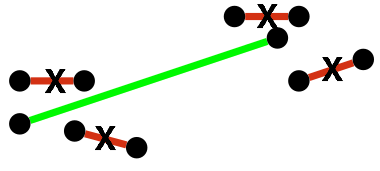
\includegraphics[scale=0.4]{imagenes/c3/Inform/Inform} 
	\caption[Ejemplo de conjunto de restricciones informativo.]{Ejemplo de conjunto de restricciones informativo. \cite{Survey:2007}}\label{fig:figure16}
\end{figure}


La informatividad se estima utilizando el conjunto de restricciones como un conjunto de test, de manera que se mide la habilidad del algoritmo para predecir las restricciones presentes en él. Formalizando, dado un conjunto de restricciones $R$ y un algoritmo $A$, obtenemos la partición $P_A$ aplicando el algoritmo al conjunto de datos de entrada especificando el conjunto de restricciones vacío. Calculamos entonces la fracción de las restricciones incumplidas por $P_A$ \cite{Survey:2007}:

\begin{equation}
I_A(R) = \frac{1}{|R|}\left[ \sum_{r \in R} unsat(r, P_A) \right] 
\end{equation}

\clearpage

Por otra parte, la \textbf{coherencia} mide el grado de concordancia dentro del propio conjunto de restricciones respecto a una métrica dada ($D$). Por ejemplo, la Figura \ref{fig:figure17} muestra dos restricciones paralelas y muy cercanas, pero de distinto tipo. Es en casos como este en los que se da una contradicción, ya que las restricciones \acf{ML} indican que la distancia entre las instancias involucradas en ellas es pequeña, mientras que las de tipo \acf{CL} deben indicar lo contrario.

\begin{figure}[!h]
	\centering
	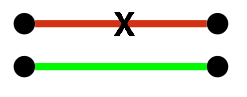
\includegraphics[scale=0.4]{imagenes/c3/Coherencia/Coher1}
	\caption[Ejemplo de conjunto de restricciones contradictorio.]{Ejemplo de conjunto de restricciones contradictorio. \cite{Survey:2007}}\label{fig:figure17}
\end{figure}

Entonces, la medida de coherencia viene dada por el grado de solapamiento que presentan las restricciones al interpretarlas como vectores en el espacio y proyectarlas sobre uno de los ejes, tal y como se muestra en la Figura \ref{fig:figure18}.

\begin{figure}[!h]
	\centering
	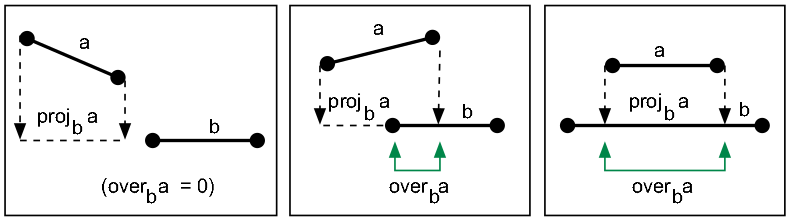
\includegraphics[scale=0.4]{imagenes/c3/Coherencia/Coher2}
	\caption[Representación de la medida de coherencia.]{Representación de la medida de coherencia. \cite{Survey:2007}}\label{fig:figure18}
\end{figure}

\section{Resumen}

El clustering con restricciones incorpora nueva información al problema del clustering original, esta viene dada en forma de especificaciones de pertenencia al mismo o a diferentes clusters sobre parejas de instancias. Las restricciones, ya sean \acf{ML}, \acf{CL}, o restricciones de distancia, son utilizadas para guiar al método de clustering que apliquemos al conjunto de datos en cuestión, en la búsqueda de la partición resultado.

Los método de clustering derivados de este concepto han demostrado ser de gran utilidad en múltiples ámbitos, así como presenta problemas que pueden ser subsanados estudiando en profundidad las restricciones a emplear para resolver cada problema.



































%\include{Chapters/Chapter01}
\cleardoublepage
%********************************************************************
% Other Stuff in the Back
%*******************************************************
\cleardoublepage%********************************************************************
% Bibliography
%*******************************************************
% work-around to have small caps also here in the headline
% https://tex.stackexchange.com/questions/188126/wrong-header-in-bibliography-classicthesis
% Thanks to Enrico Gregorio
\defbibheading{bibintoc}[\bibname]{%
  \phantomsection
  \manualmark
  \markboth{\spacedlowsmallcaps{#1}}{\spacedlowsmallcaps{#1}}%
  \addtocontents{toc}{\protect\vspace{\beforebibskip}}%
  \addcontentsline{toc}{chapter}{\tocEntry{#1}}%
  \chapter*{#1}%
}
\printbibliography[heading=bibintoc]

% Old version, will be removed later
% work-around to have small caps also here in the headline
%\manualmark
%\markboth{\spacedlowsmallcaps{\bibname}}{\spacedlowsmallcaps{\bibname}} % work-around to have small caps also
%\phantomsection
%\refstepcounter{dummy}
%\addtocontents{toc}{\protect\vspace{\beforebibskip}} % to have the bib a bit from the rest in the toc
%\addcontentsline{toc}{chapter}{\tocEntry{\bibname}}
%\label{app:bibliography}
%\printbibliography

%\cleardoublepage%*******************************************************
% Declaration
%*******************************************************
\refstepcounter{dummy}
\pdfbookmark[0]{Declaration}{declaration}
\chapter*{Declaration}
\thispagestyle{empty}
Put your declaration here.
\bigskip

\noindent\textit{\myLocation, \myTime}

\smallskip

\begin{flushright}
    \begin{tabular}{m{5cm}}
        \\ \hline
        \centering\myName \\
    \end{tabular}
\end{flushright}

%\cleardoublepage\pagestyle{empty}

\hfill

\vfill


\pdfbookmark[0]{Colophon}{colophon}
\section*{Colofón}

Este documento ha sido redactado siguiendo el estilo tipográfico \texttt{classicthesis}, desarrollado por Andr\'e Miede y Ivo Pletikosić. Dicho estilo esta inspirado en el libro sobre tipografía ``\emph{The Elements of Typographic Style}''. \texttt{classicthesis} esta disponible para \LaTeX\ y \mLyX en:

\begin{center}
	\url{https://bitbucket.org/amiede/classicthesis/}
\end{center}

\bigskip

%\noindent\finalVersionString

%Hermann Zapf's \emph{Palatino} and \emph{Euler} type faces (Type~1 PostScript fonts \emph{URW
%Palladio L} and \emph{FPL}) are used. The ``typewriter'' text is typeset in \emph{Bera Mono},
%originally developed by Bitstream, Inc. as ``Bitstream Vera''. (Type~1 PostScript fonts were made
%available by Malte Rosenau and
%Ulrich Dirr.)

%\paragraph{note:} The custom size of the textblock was calculated
%using the directions given by Mr. Bringhurst (pages 26--29 and
%175/176). 10~pt Palatino needs  133.21~pt for the string
%``abcdefghijklmnopqrstuvwxyz''. This yields a good line length between
%24--26~pc (288--312~pt). Using a ``\emph{double square textblock}''
%with a 1:2 ratio this results in a textblock of 312:624~pt (which
%includes the headline in this design). A good alternative would be the
%``\emph{golden section textblock}'' with a ratio of 1:1.62, here
%312:505.44~pt. For comparison, \texttt{DIV9} of the \texttt{typearea}
%package results in a line length of 389~pt (32.4~pc), which is by far
%too long. However, this information will only be of interest for
%hardcore pseudo-typographers like me.%
%
%To make your own calculations, use the following commands and look up
%the corresponding lengths in the book:
%\begin{verbatim}
%    \settowidth{\abcd}{abcdefghijklmnopqrstuvwxyz}
%    \the\abcd\ % prints the value of the length
%\end{verbatim}
%Please see the file \texttt{classicthesis.sty} for some precalculated
%values for Palatino and Minion.
%
%    \settowidth{\abcd}{abcdefghijklmnopqrstuvwxyz}
%    \the\abcd\ % prints the value of the length

% ********************************************************************
% Game Over: Restore, Restart, or Quit?
%*******************************************************
\end{document}
% ********************************************************************

%bibtex MemoriaTFG.aux 
